\documentclass[12pt,]{report}
\usepackage{lmodern}
\usepackage{amssymb,amsmath}
\usepackage{ifxetex,ifluatex}
\usepackage{fixltx2e} % provides \textsubscript
\ifnum 0\ifxetex 1\fi\ifluatex 1\fi=0 % if pdftex
  \usepackage[T1]{fontenc}
  \usepackage[utf8]{inputenc}
\else % if luatex or xelatex
  \ifxetex
    \usepackage{mathspec}
  \else
    \usepackage{fontspec}
  \fi
  \defaultfontfeatures{Ligatures=TeX,Scale=MatchLowercase}
\fi
% use upquote if available, for straight quotes in verbatim environments
\IfFileExists{upquote.sty}{\usepackage{upquote}}{}
% use microtype if available
\IfFileExists{microtype.sty}{%
\usepackage{microtype}
\UseMicrotypeSet[protrusion]{basicmath} % disable protrusion for tt fonts
}{}
\usepackage[margin = 1.2in]{geometry}
\usepackage{hyperref}
\PassOptionsToPackage{usenames,dvipsnames}{color} % color is loaded by hyperref
\hypersetup{unicode=true,
            colorlinks=true,
            linkcolor=blue,
            citecolor=Blue,
            urlcolor=cyan,
            breaklinks=true}
\urlstyle{same}  % don't use monospace font for urls
\usepackage{natbib}
\bibliographystyle{plainnat}
\usepackage{graphicx,grffile}
\makeatletter
\def\maxwidth{\ifdim\Gin@nat@width>\linewidth\linewidth\else\Gin@nat@width\fi}
\def\maxheight{\ifdim\Gin@nat@height>\textheight\textheight\else\Gin@nat@height\fi}
\makeatother
% Scale images if necessary, so that they will not overflow the page
% margins by default, and it is still possible to overwrite the defaults
% using explicit options in \includegraphics[width, height, ...]{}
\setkeys{Gin}{width=\maxwidth,height=\maxheight,keepaspectratio}
\IfFileExists{parskip.sty}{%
\usepackage{parskip}
}{% else
\setlength{\parindent}{0pt}
\setlength{\parskip}{6pt plus 2pt minus 1pt}
}
\setlength{\emergencystretch}{3em}  % prevent overfull lines
\providecommand{\tightlist}{%
  \setlength{\itemsep}{0pt}\setlength{\parskip}{0pt}}
\setcounter{secnumdepth}{5}
% Redefines (sub)paragraphs to behave more like sections
\ifx\paragraph\undefined\else
\let\oldparagraph\paragraph
\renewcommand{\paragraph}[1]{\oldparagraph{#1}\mbox{}}
\fi
\ifx\subparagraph\undefined\else
\let\oldsubparagraph\subparagraph
\renewcommand{\subparagraph}[1]{\oldsubparagraph{#1}\mbox{}}
\fi

%%% Use protect on footnotes to avoid problems with footnotes in titles
\let\rmarkdownfootnote\footnote%
\def\footnote{\protect\rmarkdownfootnote}

%%% Change title format to be more compact
\usepackage{titling}

% Create subtitle command for use in maketitle
\newcommand{\subtitle}[1]{
  \posttitle{
    \begin{center}\large#1\end{center}
    }
}

\setlength{\droptitle}{-2em}
  \title{}
  \pretitle{\vspace{\droptitle}}
  \posttitle{}
  \author{}
  \preauthor{}\postauthor{}
  \date{}
  \predate{}\postdate{}

\usepackage[section]{placeins}
\usepackage{caption}
\usepackage{fancyhdr}
\usepackage{setspace}
\usepackage{chngcntr}
\usepackage{microtype}
\usepackage{booktabs}
\usepackage{graphicx}
\usepackage{epigraph}
\usepackage[inline]{enumitem}
\usepackage[flushleft]{threeparttable}
\usepackage{perpage}
\usepackage{hyperref}
\usepackage[utf8]{inputenc}
\MakePerPage{footnote}
\onehalfspacing

\begin{document}

\pagenumbering{gobble}

\begin{centering}

\vspace{3 cm}

\Huge

{\bf Multimorbidity and Access to Social Care: exploiting emerging administrative data sources in Scotland}

\vspace{3 cm}

\Large
David Alexander Gunn Henderson

\vspace{3 cm}


\normalsize
Submitted in partial fulfilment of the requirements of the degree of ...

Month Year

\vspace{3 cm}

\normalsize
College of Social Sciences

\normalsize
University of Glasgow

\end{centering}

\newpage

\pagestyle{fancy}

\fancyhead[LE,RO]{} \fancyhead[LO,RE]{}
\renewcommand{\headrulewidth}{0.4pt} \renewcommand{\footrulewidth}{0pt}

\pagenumbering{roman}

\section*{Abstract}\addcontentsline{toc}{section}{Abstract}

Blad de Blah blah blah. I may play about with centering and italicised
styles here

\newpage

\fancyhead[CO,CE]{Table of Contents} \setcounter{tocdepth}{2}
\tableofcontents

\newpage

\fancyhead[CO,CE]{List of Tables}
\addcontentsline{toc}{section}{List of Tables} \listoftables

\newpage

\fancyhead[CO,CE]{List of Figures}
\addcontentsline{toc}{section}{List of Figures} \listoffigures

\newpage

\section*{Acknowledgements}

\fancyhead[CO,CE]{} \addcontentsline{toc}{section}{Acknowledgements}

Again maybe play about with centering and layout.

How about a nice quotation at the end???

\newpage

\section*{Declaration}

\fancyhead[CO,CE]{} \addcontentsline{toc}{section}{Declaration}

I declare, except where explicit reference is made to the contribution
of others, that this thesis is the result of my own work and has not
been submitted for any other degree at the University of Glasgow or any
other institution.

Printed Name: David Henderson

Signature:

\newpage

\pagenumbering{arabic}

\newpage

\fancyhead[CO,CE]{Chapter 1. Introduction}

\chapter{Introduction}\label{ch:intro}

Integration of health and social care became law in Scotland on 1st
April 2016. Reflects patterns across the developing world to restructure
health services to cope with demands of an ageing population.

Social Care of increasing policy (and political) importance. Link to
healthcare (and demands on health services) becoming increasingly
apparent (increase delayed discharge etc).

This, in part, due to long-term conditions now major burden of global
disease (replacing infectious diseases). Large proportions of population
have multimorbidity (OECD) which has a number of negative outcomes
including mortality and health care use.

Association of multimorbidity and social care use is unknown.

PhD funding from Scottish Government to assess these topics. (2020
vision and other policy link)

Important part of the funding to link administrative data sources in
order to identify the benefit of this process. \emph{Measurement of
social (or LTC) is improtant for a number of reseons - OECD(2013) page
18, Care co-ordination (integration) is not measured well pp 76,
administrative databases potential to help these problems plus ideas for
outcome measures pp 76 \& 79, pp81 obstacles to data collection
(overcome by data linkage in Soctland??}

(Need WHO policy outlines and other suitable high-level policy docs in
this section)

Many countries, including the United Kingdom (UK), have recently seen
policies implemented that aim to integrate the provision of health and
social care services \citep{RN234, RN362, RN262}. In addition to
reducing variations in the provision of care across geographic areas,
these policies hope to save public money by reducing unplanned
admissions and delayed discharges from hospital whilst also improving
the quality of services for individuals \citep{RN232, RN266, RN406}.

The World Health Organisation \citeyearpar{RN320} cites relative
inequalities in improvements of health and life expectancy, within and
between countries, as justification for recommended structural change to
healthcare \citep{RN320}. The paradigm shift in the method of service
delivery is suggested in response to increasing long-term, chronic
conditions forming the major burden of care worldwide. Integrating
health and social care services and increasing primary care spend are
cited as two potential ways of facilitating this shift in focus
\citep{RN320}.

Policies introduced that facilitate integration of services have been
implemented despite little evidence to suggest they will have the
desired effect
\citep{RN367, RN369, RN234, RN233, RN321, RN362, RN366, RN260}. The
continued drive to integrate services does, however, implicitly
acknowledge that health and social care services are linked. How these
services interact at the individual level and whether differing levels
of provision in each service affects the other is not well understood
\citep{RN361, RN205, RN406}.

Until recently many local authorities had attempted to protect
front-line services, such as social care, from austerity cuts
\citep{RN117}. However, given continued year-on-year reductions and a
further 7.2\% cut to local authority spending in 2016/2017
\citep{RN251}, the ability to protect social care from reductions in
spend becomes less likely. Decreased local government budgets across the
UK and Scotland since 2010 have affected those living in the poorest
areas hardest \citep{RN117, RN235}. If social care budgets decrease
further, the question of whether the most deprived areas will feel these
cuts most is of grave importance.

\section{Aims and Objectives}\label{sec:intro-aims-and-obs}

Does an inverse \emph{social} care law exist? i.e.~Does the allocation
of resources (via funding formulae) to Local Authorities negatively
impact on those areas with higher need?

Furthermore, does access to social care vary across Local Authorities -
is there a ``postcode lottery'' in terms of service provision i.e.~does
application of eligibility criteria depend on where you live?

Is multimorbidity status associated with levels of social care provided
within \emph{and} across local authorities? What is the best way to
measure multimorbidity? Do clustering techniques offer a better
understanding of this phenomenon?

Important to understand how access to social care influences health care
use and mortality - do those with multimorbidity and social care have
different outcomes from those with multimorbidity and no social care?

The thesis has both substantive and methodological aims. Substantively,
it aims to contribute to the debate surrounding health and social care
integration by looking specifically at a group that are likely to be
regular users of both health and social care services, i.e.~those with
multimorbidity. Methodologically, the thesis aims to contribute to
efforts to improve the exploitation of administrative data as a means to
analyse public service performance and effectiveness.

Aims of the project are:-

\begin{enumerate}[noitemsep]
\item Describe and compare social inequalities in the use of social care services using linked health and social care data.
\item Explore the effects of social care use for those with multimorbidity on 
\begin{enumerate} 
\item unscheduled health care use and
\item mortality. 
\end{enumerate}
\end{enumerate}

The objectives of the project are:-

\begin{enumerate}[noitemsep]
\item To assess how access to social care services varies for people with multimorbidity, especially by socioeconomic status.  
\item To assess the impacts of social care service use on health service use and health outcomes for people with multimorbidity, where possible exploiting geographic differences in social care as "natural experiments".
\item To make recommendations for policy on the future of integration of health and social care services based on these results.
\item To assess tho what extant measures of multimorbidity and of health and social care service use can be operationalised using existing linked health and social care administrative data.
\item To make recommendations to policy makers on administrative data collections. 
\end{enumerate}

\section{Scientific contribution}\label{sec:intro-contribution}

Explicit description of what thesis adds to knowledge

\section{Conventions}\label{sec:intro-conventions}

Outline definitions

\begin{itemize}
\tightlist
\item
  Social care refers to Adult social care (with link to subsection
  \ref{subsec:access-sc-defs})
\item
  Multimorbidity and morbidity burden as opposed to comorbidity (with
  link to subsection \ref{subsec:mm-defs})
\end{itemize}

\FloatBarrier
\newpage
\fancyhead[CO,CE]{Chapter 2. Literature Review}

\chapter{Literature Review}\label{ch:lit-review}

\section{Introduction}\label{sec:lit-review-intro}

This chapter identifies and summarises academic and policy literature
relevant to the thesis. Literature regarding a) access to social care,
b) health and social care interaction and c) multimorbidity is
presented. As the main research is conducted with Scottish data, there
is appropriate focus in the structures and policies regarding health and
social care in this country. However, this is placed in the wider
context of the UK and developed world.

The chapter is organised in three parts following the main themes listed
above. Section \ref{sec:access-sc} focuses on social care from a number
of perspectives; varying definitions of the term, differing
international models, social theory of eligibility and resource
allocation, and finally the impact on health inequalities.

Section \ref{sec:hsc-interaction} outlines the policy framework
regarding health and social care services, how these services are funded
and delivered, and why they are linked. It then describes the
legislation that made health and social care integration law in Scotland
before reviewing empirical evidence of the nature of the interaction
between health and social care services.

Section \ref{sec:mm} describes why multimorbidity is important in the
context of health and social care integration and then provides an
overview of academic literature and policy documents regarding
multimorbidity and its definitions, measurement, and epidemiology.

\section{Access to Social Care}\label{sec:access-sc}

\subsection{Definitions}\label{subsec:access-sc-defs}

As in the case of multimorbidity, discussed in section
\ref{subsec:mm-defs}, there is no internationally (or nationally)
accepted definition of social care. Indeed, the difference between what
is social care and what is health care has no clear line of demarcation
resulting in local variation in provision of services \citep{RN371}. The
Organisation for Economic Co-operation and Development (OECD) and the
European Union (EU) jointly published a report on Long Term Care (LTC)
for older people discussing much of what may be described in the UK as
social care. In the report, LTC is defined as,

\begin{quotation}
"... a range of services required by persons with a reduced degree of functional capacity, physical or cognitive, and who are consequently dependent for an extended period of time on help with basic activities of daily living (ADL). This "personal care" component is frequently provided in combination with help with basic medical services such as "nursing care" (wound dressing, pain management, medication, health monitoring), as well as prevention, rehabilitation or palliative care. Long-term care services can also be combined with lower level care related to “domestic help” or help with instrumental activities of daily living (IADL)." 
\end{quotation}

\citep[pp38]{RN406}

A recent NICE guideline \citeyearpar{RN150} addressing social care needs
for older people with multiple chronic conditions used a definition
provided in the UK Health and Social Care Act \citeyearpar{RN149}:-

\begin{quotation}
    ““Adult social care”—
    (a) includes all forms of personal care and other practical assistance provided for individuals who, by reason of age, illness, disability, pregnancy, childbirth, dependence on alcohol or drugs, or any other similar circumstances, are in need of such care or other assistance, but 
    (b) does not include anything provided by an establishment or agency for which Her Majesty’s Chief Inspector of Education, Children’s Services and Skills is the registration authority under section 5 of the Care Standards Act 2000.”
    (The Health and Social Care Act  2012 c7, Part 3, Chapter 1, Section 65, Subsection 4)
\end{quotation}

The NICE guideline \citeyearpar{RN150} advises that social care planning
for people with multimorbidity should include holistic assessment of
biopsychosocial factors including sexual, spiritual, cultural, and
communication needs. It should also consider access to leisure and
social activities whilst incorporating issues regarding mobility and
transport. Specifically, the guideline cites; self-care, taking
medicines, learning, volunteering, maintaining a home, financial
management, employment, socialising with friends and hobbies as
activities that all patients should be able to take part in should they
wish to and social care assessment should assess the ability of the
individual to achieve this.

A more succinct definition of social care is used in a report to the
Minister for Care Services at the UK Department of Health, :-

\begin{quotation}
    "The group of services that provide personal care and support to people in social situations – such as family; the community; a communal setting; to help them achieve independence and to promote their positive contribution as citizens." Platt 
\end{quotation}

\citeyearpar[pp.~4]{RN154}

Huxley et al. \citeyearpar{RN153} are critical of this service-based
definition and argue that social care is intended to improve general
well-being for those that are in need. As quality of life is an
important factor of well-being, Huxley et al. \citeyearpar{RN153} argue
that wider issues regarding environment and the quality of public and
private services also play an important role in social care. Indeed,
Daly and Lewis \citeyearpar[pp.287]{RN146} argue that social care is
``\ldots{}an activity and set of relations lying at the intersection of
state, market, family (and voluntary sector) relations.''

This view is reflected in an aspirational constitution for social care
published by an independent, cross-party think-tank \citep{RN136}. The
authors argue that all citizens should have an equal ability to live and
control a full and active life. Where this is not possible the state
should have a duty to provide the necessary help, in whatever form that
is required, to individuals who require it.

A more clearly defined concept is that of \textit{personal care} which
has been provided for free in Scotland since 2002. The legislation
introduced by the then Scottish Executive necessitated a clear
definition and constitutes six dimensions \citep[pp.256]{RN373}.

\begin{itemize}[noitemsep]
\item personal hygiene: washing etc.  
\item personal assistance: help with dressings, prostheses etc.  
\item continence management: toileting, catheter management etc.  
\item food and diet: help with eating, food preparation etc.  
\item problems of immobility:  
\item simple treatments: help with medicines, creams, oxygen therapy etc. 
\end{itemize}

Personal care is, however, only one aspect of social care provision and
clear definitions of other services provided to individuals are lacking.
Nevertheless, the definitions of social (or long-term) care above all
highlight services that are required to aid with an individual's
functional or cognitive needs.

A final definition provided by Colombo et al\citeyearpar{RN414} will be
used for the purposes of this thesis:-

\begin{enumerate}[noitemsep, label={\alph*)}]
\item a group of services such as; skilled nursing care, social work, personal care, medical equipment \& technologies, and therapies. Delivered by,   
\item a range of  professionals such as; nurses, low-skilled carers, or allied health professionals. In,  
\item various locations such as; at home, in an institution, or via community care.
\end{enumerate}

This definition clearly captures the broad range of services that can be
associated with social care that are only partially provided in other
definitions. It acknowledges that social care can include a number of
components including personal, nursing care and help with other domestic
activities, and articulates the variety of settings where this can take
place. Whilst it is common in Europe to describe ``Long-term care'' in
relation to these services, this thesis will refer to ``social care'' as
this is the most commonly used term in the UK. Furthermore, unless
stated otherwise, reference to social care in this thesis will be with
regard to care received by adults over the age of 65.

\subsection{International models of social care}\label{subsec:access-sc-models}

There are four ways in which social care can be provided to those in
need; informally via family or community, formally via voluntary
non-profit organisations, formally via the state, or formally via
for-profit organisations \citep{RN346}. In Europe, increasing demand
from users has led to many welfare systems being unable to adequately
provide care \citep{RN344, RN414}. Changes in demography, the labour
market, democracy, and values have all contributed to the increasing
pressure on care services \citep{RN406, RN342, RN414}. There is wide
consensus that lower birth rates and higher proportions of older people
mean that a gap has emerged in the number of adult children able to
provide informal care to their parents
\citep{RN342, RN343, RN344, RN346, RN345, RN414}. Traditionally,
informal care was provided by women. As gender equality improves, more
women are employed outwith domestic circumstances which also reduces the
pool of informal social care available \citep{RN342}. Anttonen
\citeyearpar{RN342} also cites changes in societal attitudes from
``familism'' to ``individualism'' as having an impact on informal care
resources. These combined factors mean that formal care services are
increasingly required to provide social care. Pressures on these
services has seen increased discussion and comparison of models of care
across Europe over the last 20 years \citep{RN347, RN348, RN346, RN349}.

In a report for the OECD, Colombo et al \citeyearpar{RN414} categorised
the varying models of social care into three main groups with
subdivisions as shown in Table \ref{tab:oecd-soc-care}.

\begin{table}[h]
  \centering
  \caption{Models of social care in OECD countries adapted from Colombo et al (2011)}
  \label{tab:oecd-soc-care}
  \scalebox{0.7}{
    \begin{threeparttable}
      \begin{tabular}{@{}ll@{}}
        \toprule
          \textbf{Model} & \textbf{Countries where employed} \\ \midrule
          \textbf{Universal coverage} &  \\
          a) tax based & Norway, Sweden, Denmark, Finland \\
          b) public long-term insurance & Germany, Japan, South Korea,                      Netherlands, Luxembourg \\
          c) health system & Belgium \\
          \textbf{Mixed systems} &  \\
          a) parallel universal schemes & Scotland, Italy, Czech Republic,                 Poland \\
          b) income-related universal benefit or subsidy & Ireland, Australia,              Austria, France \\
          c) mix of universal and means-tested (or no) benefit & Switzerland,               New Zealand, some Canadian Provinces, Spain, and Greece\tnote{1} \\
          \textbf{Means-tested safety net} & England, USA \\
          \bottomrule
          \end{tabular}
          \begin{tablenotes}
        \item[1] Spain and Greece have less well developed formal care                    services
      \end{tablenotes}
  \end{threeparttable}
  }
\end{table}

Universal models of social care are characterised by; a) a single system
being in place for delivery of services, b) nursing \textit{and}
personal care are provided for all individuals meeting defined
eligibility criteria, and c) some form of charge is levied on
service-users \citep{RN414}. Three subdivisions of universal coverage
social care models are identified in this classification.

The tax-based universal models, also known as the Nordic model of care,
have strong local-government influence in both the raising of funds and
delivery of services \citep{RN414, RN348, RN346, RN349}. Overall
responsibility remains with national government which also contributes
funds, often dependent on local population need and structure
\citep{RN414}. Public long-term insurance schemes are mandatory in the
countries that employ them, although the age at which citizens begin to
contribute varies (e.g.~only over 40s contribute in Japan)
\citep{RN414, RN413, RN407}. These models have found it increasingly
difficult to fund provision and have either increased user-payments or
decreased coverage in recent years \citep{RN345, RN413, RN407}. In
Belgium, social care is viewed as a health risk and is financed through
the health system with a cap on user-contribution. This results in a
medical (rather than social) model of care delivery, mostly provided by
nurses \citep{RN414}.

In contrast to universal models described above where a single system is
in place for social care delivery, mixed social care systems employ
either; a) universal coverage via different sources/sectors or b) a
mixture of universal and means-tested benefits \citep{RN414}. Whilst
acknowledging the wide variation in systems, Colombo et al
\citeyearpar{RN414} identify three subdivisions of mixed system models
of social care as shown in table \ref{tab:oecd-soc-care}.

Parallel universal schemes provide social care via two or more sectors
(e.g.~nursing care via health provider and personal care from a
non-healthcare source) \citep{RN414}. Major differences exist between
countries in how this is delivered in practice with varying degrees of
coverage. Income related universal benefits provide needs-based
universal coverage of social care but benefits received vary according
to income \citep{RN414}. France provides a good example of this system
where cash benefits are need \textit{and} income based - benefits are
paid at six levels of dependency, those with higher incomes are paid
proportionally less and top-up care costs themselves
\citep{RN414, RN420}. The final subdivision of mixed social care models
has some universal entitlements provided alongside means-tested services
e.g.~free provision of nursing care with means-testing for personal
care.

Colombo et al \citeyearpar{RN414} include Spain and Greece in this final
subdivision of mixed social care models but note these countries have
formal care systems that are much less developed than elsewhere in the
OECD. Sometimes referred to as the Mediterranean model, informal care
from family and other sources constitutes the main form of social care
in these countries \citep{RN348, RN346, RN349}. As this role is
traditionally carried out by women, the Mediterranean model has
attracted criticism from a feminist perspective \citep{RN346}.

The final model in Colombo et al's \citeyearpar{RN414} classification of
social care in OECD countries is the means-tested safety net model
(Table \ref{tab:oecd-soc-care}). In this model only those below a
pre-determined threshold are entitled to state-provided social care.
Despite the free provision of health care and some non-means-tested
benefits, England is included in this category in the report. Presumably
this is due to the fact that state support in a residential home in
England is provided only after an individual has depleted both income
\textit{and} assets below a threshold \citep{RN414}, a system not seen
in other countries
\footnote{A cap of approximately £72,000 total contribution was to be introduced in 2016 (Eleftheriades et al., 2013)}
\citep{RN420}.

Of the three models of social care described in this section, universal
systems have a number of advantages over the other two
\citep{RN414, RN420}. Sharing the burden of social care provision among
the entire population, either via general taxation or mandatory
insurance schemes, results in a reliable, predictable source of finance
enabling states to plan more effectively \citep{RN414, RN420, RN413}.
Mixed systems of social care can still result in considerable costs for
those that require care, whereas the costs to individuals in the
means-tested system can be ``catastrophic'' \citep[pp240]{RN414}. The
means-tested system can also be perceived as unfair for those that need
to sell assets (such as a house) to pay for care, particularly when
there is variation in eligibility criteria within countries
\citep{RN414, RN420, RN421, RN407, RN413}. A particular advantage of a
universal social care system is that it,

\begin{quotation} 
"...generally reduces utilisation of more expensive health care services and professionals (e.g. hospital care, doctors) for long-term care needs, for example by making "social hospitalisation" of frail people with [social care] needs more difficult." 
\end{quotation}

\citep[pp.222]{RN414}

Given the pressures on state budgets and the desire to adequately fund
care services, this seems a particularly useful benefit of the universal
coverage model of social care.

Disadvantages of universal systems are that they are generally more
expensive to the state than other models of social care and can reduce
the amount of informal care provided by relatives for elderly family
\citep{RN414, RN407}. The comprehensiveness of coverage can be
over-burdensome for the state with a number of countries recently having
to cut service or increase user-contributions to compensate for
increasing demand \citep{RN345, RN421, RN407, RN413}.

A recent examination of the effects of the 2008 financial crisis on the
way social care is delivered across Europe suggests that the
distinctions between social care models is beginning to blur
\citep{RN343}. There is evidence those with more comprehensive coverage
are reducing levels of care whilst those with less coverage are
increasing provision \citep{RN414}.

\begin{figure}[h]
  \centering
  \caption{Older recipients of long-term care services as a share of the over 65 population, 2008}
  \label{fig:oecd-comparison}
    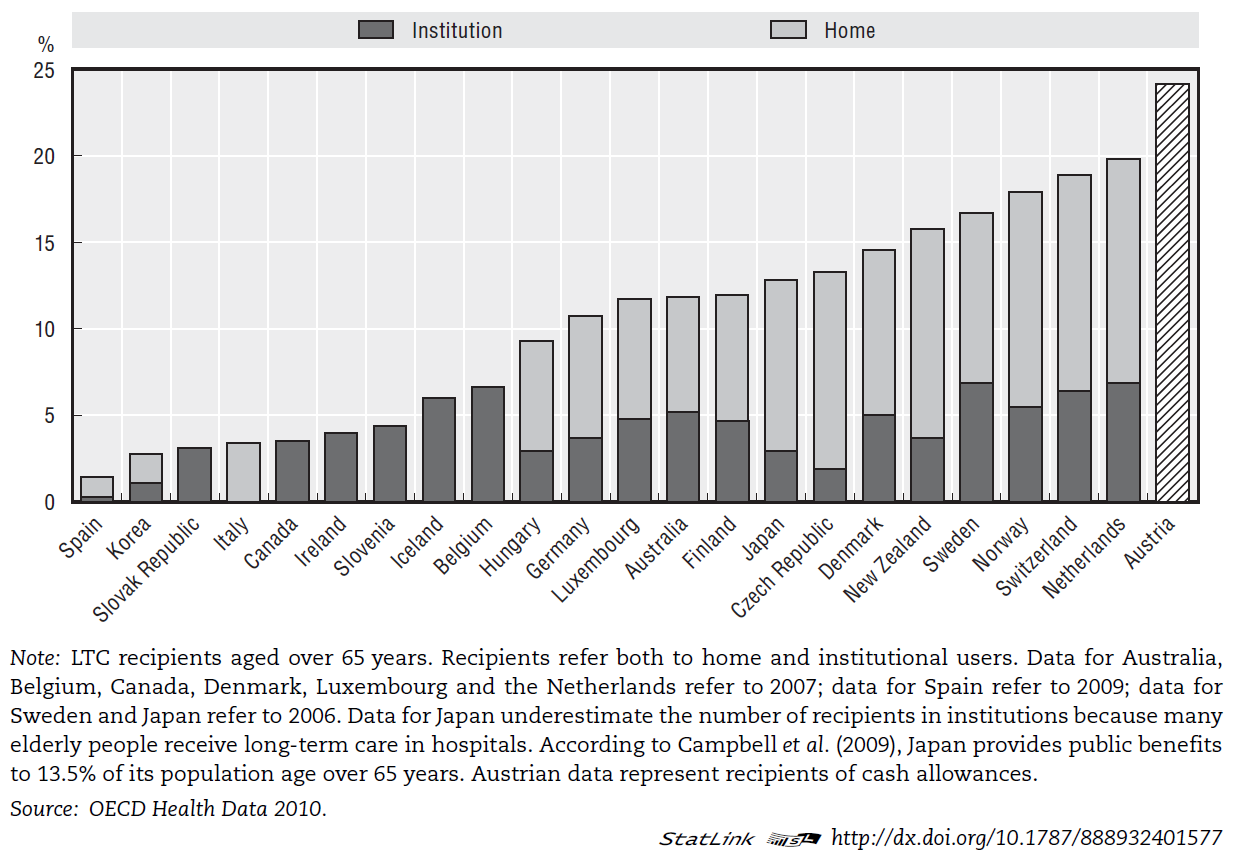
\includegraphics[width=0.8\textwidth]{figures/oecd-comparison.PNG}
\end{figure}

Given the marked variations in how social care is funded and delivered
across countries, it may be expected that there are also marked
variations in levels of access and utilisation. Colombo et al
\citeyearpar{RN414} produced a chart (shown in figure
\ref{fig:oecd-comparison}) derived from OECD data that shows the
proportion of over 65s receiving some form of social care across
countries for which data is provided. The chart shows that having a
universal or mixed system of social care provision (as described above)
does not absolutely influence the number of people receiving care. For
example, South Korea employs a universal (insurance-based) system and
has one of the lowest proportions of older people receiving care,
whereas Switzerland has one of the highest whilst employing a mixed
system involving some universal and some means-tested benefits. This
suggests that allocation of resources and eligibility criteria set
within countries are likely to be more important in determining access
to social care than any particular system of care delivery.

\subsection{Access to Social Care - Social Theory of Eligibility}\label{subsubsec:eligibility-theory}

\setlength{\epigraphwidth}{0.8\textwidth}
\epigraph{"...the \textit{criteria} under which a given individual is eligible for publicly funded support for long-term care, and for how much support the individual is eligible, and the \textit{processes} involved in selecting from the general population those who receive this support and determining for how much support each person is eligible"}{\textit{[Eleftheriades and Wittenberg, 2013, pp.2}}

Two social theories on how eligibility for public services are
determined will be discussed in this subsection; street-level
bureaucracy and candidacy.

The term street-level bureaucracy is generally credited to Michael
Lipsky and his book of the same name \citeyearpar{RN174}, along with its
more recent revision \citep{RN430}. The theory investigates the extent
to which front-line public service workers exercise discretion in which
individuals of the general public are eligible to access any given
service - doing so from a position of authority \citep{RN430}. As a
result, street-level bureaucrats control, ``\ldots{}the nature, amount,
and quality of benefits and sanctions provided by their agencies.''
\citep[pp.13]{RN430}. Using the term, ``street-level'' suggests that the
theory is concerned with power, where it resides, and who wields it
\citep{RN428}. Street level bureaucrats can be teachers, police
officers, nurses, social workers, or any other worker providing a public
service \citep{RN428} and their ``\ldots{}decisions\ldots{}, the
routines they establish, and the devices they invent to cope with
uncertainties and work pressures effectively \textit{become} the public
policies they carry out'' \citep[pp.xiii]{RN430}.

Evans\citeyearpar{RN424} and Ellis \citeyearpar{RN426} both provide a
critique of street-level bureaucracy that suggests the theory needs to
be augmented to take into account new structures of public services,
particularly in social work, that place greater autonomy with managers
than front-line workers. They argue that these new structures mean
workers who deal face-to-face with public service users have less
discretion about eligibility criteria and are more likely to have to
justify eligibility decisions to senior members of staff who now wield
more power in terms of service access.

Empirically exploring the effects of street-level bureaucracy poses a
number of methodological problems \citep{RN428}. The use of large sample
surveys of public sector workers investigating their views and how they
make decisions is one way (e.g. \citep{RN427}). However Lipsky
\citeyearpar{RN430} and Hupe et al \citeyearpar{RN428} agree that
qualitative interview techniques with public sector workers in their own
workplace is the best way to fully understand how street-level
bureaucracy impacts on front-line services.

The term ``candidacy'' was first used by Dixon-Woods et al
\citetext{\citeyear{RN438}; \citeyear{RN437}} to form a concept of how
vulnerable individuals identified themselves as being eligible for a
particular health service or intervention given for particular illnesses
or health conditions. The theory was further explored and augmented by
Mackenzie et al \citetext{\citeyear{RN84}; \citeyear{RN434}} in relation
to access and utilisation of all public services as a way to explore
concerns about unequal distribution of uptake.

The theory argues that there are a number of social and cultural factors
that contribute to an individual's interpretation of their eligibility
for a given service and is based on a seven-stage model as shown in
Table \ref{tab:candidacy}

\begin{table}[h]
\centering
\caption{Seven stage model of candidacy}
\label{tab:candidacy}
\resizebox{\textwidth}{!}{%
\begin{tabular}{@{}ll@{}}
\toprule
\multicolumn{1}{l}{\textbf{Stages of candidacy}} & \multicolumn{1}{c}{\textbf{Description of stage}} \\ \midrule
\begin{tabular}[c]{@{}l@{}}Self-identification of \\ candidacy\end{tabular} & \begin{tabular}[c]{@{}l@{}}Process by which individuals come to view themselves as legitimate \\ candidates for particular services\end{tabular} \\ \hline
\begin{tabular}[c]{@{}l@{}}The availability and \\ accessibility of services\end{tabular} & \begin{tabular}[c]{@{}l@{}}Knowing how to make contact with appropriate services in relation to \\ identified candidacy\end{tabular} \\ \hline
Permeability of services & \begin{tabular}[c]{@{}l@{}}Includes the level of explicit and implicit gate-keeping within a service and \\ the complexity of its referral systems; in addition it refers the\\ "cultural alignment" between users and services\end{tabular} \\ \hline
\begin{tabular}[c]{@{}l@{}}Appearing at services and \\ asserting candidacy\end{tabular} & \begin{tabular}[c]{@{}l@{}}The work that an individual must do to assert their candidacy in an\\ interaction with a service professional\end{tabular} \\ \hline
\begin{tabular}[c]{@{}l@{}}Professional decision \\ making\end{tabular} & \begin{tabular}[c]{@{}l@{}}Candidacy as expressed by service user is validated or otherwise by service \\ professional. This influences future offers of service\end{tabular} \\ \hline
\begin{tabular}[c]{@{}l@{}}Offers of and resistance to\\ services\end{tabular} & \begin{tabular}[c]{@{}l@{}}Service may be appropriately or inappropriately offered by a professional and\\ this may, or may not, be acted on by service user\end{tabular} \\ \hline
\begin{tabular}[c]{@{}l@{}}Operating conditions and local \\ production of candidacy\end{tabular} & \begin{tabular}[c]{@{}l@{}}Incorporates factors that influence decision about future service provision \\ (e.g. resources) and the relationship that develops between service users and \\ professionals over a number of encounters\end{tabular} \\ \bottomrule
\end{tabular}%
}
\end{table}

This is a much broader theory than that of street-level bureaucracy and
focusses on the barriers and enablers individuals face/use when
accessing services. It could be argued that candidacy includes the
concept of street-level bureaucracy in the fifth and sixth stages of the
model shown in table \ref{tab:candidacy}. ``professional decision
making'' and ``offers of and resistance to services'' are areas where an
interface between a service user and service professional takes place -
much like the interactions described by Lipsky.

Investigating candidacy as a theory empirically again appears to be best
served using qualitative methods. The complex and dynamic nature of
candidacy suggests identifying meaningful quantitative measures are
unlikely. Both Dixon-Woods et al
\citetext{\citeyear{RN438}; \citeyear{RN437}} and Mackenzie et al
\citetext{\citeyear{RN84}; \citeyear{RN434}} employed critical
interpretive synthesis in their studies.

Both of the social theories described in this subsection deal with the
concept of eligibility and how, in the case of street-level bureaucracy,
professionals exercise discretion on access to service and, in the case
of candidacy, how service-users identify whether they are eligible and
offer themselves for a service in the first place. Both theories
describe complex interactions between individuals across an eligibility
criteria barrier. The next section describes in detail this eligibility
barrier in relation to social care in the UK, firstly from a Scottish
perspective and then more broadly in the wider UK.

\subsection{Access to Social Care - Eligibility in the UK}\label{subsubsec:eligibility-uk}

\epigraph{"It is through the eligibility criteria that resources are rationed, that is "need" is equated with "resources available". This mechanism severely limited the idea that provision could be determined either by need or by the right to services."}{\textit{[Sharkey, 2006, pp.10]}}

In Scotland, access to social care is needs-tested via assessment
carried out by a social worker. The criteria for social care delivery,
therefore, has a very important part to play in how services are
accessed.

In 2010 the Scottish Government published a report identifying a
strategy for the policy of self-directed support \citep{RN171}. The
report was written in conjunction with the Convention of Scottish Local
Authorities~(COSLA) and included the recommendation that the National
Eligibility Framework developed by the Sutherland review into free
personal and nursing care \citeyearpar{RN172} should be applied across
all social care services. The framework has four criteria for assessing
risk in relation to a person's care needs: critical, substantial,
moderate and low \citep{RN184}. The critical and substantial levels of
risk indicate social care needs should be addressed immediately or
imminently, whereas a moderate level of risk may indicate either some or
no services being required. There is \textit{no explicit description} of
severity or which care needs fall into each category and in practice
each local authority sets the criteria and decides at which level of
risk they will provide social care \citep{RN170}.

Equity of access to services is directly influenced by an eligibility
framework. Indeed, the strategy for self-directed support
\citep[pp.20]{RN171} acknowledges this and states that such a framework
``\ldots{}can result in resources being narrowly focused on individuals
with acute needs.'' However, the report goes on to state that growing
demand and finite resources requires some form of eligibility assessment
but this should not have a disproportionate effect on any one group of
people requiring care.

The eligibility framework allows each local authority to set thresholds
for access to care in line with local priorities and resources. This has
the effect that access to services varies across differing council
areas. The potential for regional variation is again acknowledged by the
strategy for self-directed support \citep[pp.20]{RN171} which states
that, ``\ldots{}further work will be undertaken by the Scottish
Government and COSLA to assess whether there is merit in establishing
national thresholds for access to formal support across all client
groups.''

Acknowledgement of problems with eligibility criteria and the promise of
``further work'' to be undertaken by the Scottish Government and COSLA
is repeated in practitioner guidance on Self-Directed Support published
in 2014 \citep[pp.19]{RN170} and that , ``\ldots{}it remains the case
that local authorities should operate eligibility criteria to determine
whether or not an individual assessed as having social care needs can
access formal support and if so, which of their needs are to be met by
that support.''

Data is not available on levels of care provided by LAs for each of the
National Eligibility Framework criteria or for the threshold that each
LA provides care at. The Scottish Government collects an annual report
of eligibility and waiting times for the first quarter of the year. A
recent report \citep{RN184} provides information on the time individuals
had to wait to receive assessment and the time individuals had to wait
to receive care in the period January-March for the preceding five
years. However, no absolute numbers of people in each category is
provided.

The Scottish National Eligibility Framework has striking similarities to
that formerly used in England and described in Fair Access to Care
Services (FACS) produced by the Social Care Institute for Excellence
(SCIE) \citeyearpar{RN138}. Exactly the same nomenclature is used to
describe the eligibility categories of need. Newton and Browne
\citeyearpar{RN163} critiqued a previous version the FACS guidance and
found similar issues to those raised above regarding regional variations
in service and concentration of services on those with the highest need.
Their paper describes further issues with access to social care in the
context of social theory described by Lipsky \citeyearpar{RN174} and
``street-level bureaucracy'' (discussed in section
\ref{subsubsec:eligibility-theory}) where intentional and unintentional
judgement of entitlement by social care workers have an impact on
whether an individual receives care or not. Newton and Browne
\citeyearpar{RN163} also make the assertion that health and social care
has never been accessed equitably by arguing that those with a greater
ability to articulate needs and negotiate access are more likely to gain
access to services. Although no citation is provided to back-up this
argument, it has certainly been described elsewhere \citep{RN118} and
sits well in the broader discussion of inequitable access to services
\citep{RN116, RN175, RN120} (discussed further in section
\ref{subsubsec:theory-resources}).

In England, the Care Act \citeyearpar{RN176} aimed to remove regional
variations in eligibility in access to social care by imposing national
minimum thresholds that local authorities would have a statutory
obligation to provide. The Care Act also aimed to ensure local
authorities provided care, ``\ldots{}as early as possible to help
maintain well-being and independence, and potentially delay a situation
where longer-term care and support might be required.''
\citep[pp.2]{RN169}. The minimum criteria for being eligible for care
involves an individual having needs that impairs their ability to meet
two or more of a designated list of outcomes (e.g.~managing and
maintaining nutrition or maintaining hygiene) \citep{RN169} and is set
by the Secretary of State for Health \citep{RN177}.

In practice, the most likely outcome is that the minimum threshold that
local authorities will have to provide care will be similar to the
``critical'' level of the National Eligibility Framework previously used
in the FACS guidance \citep{RN173, RN177} (and similar to that used in
Scotland). This will legalise a shift that has already been occurring in
England where fewer numbers of LAs are providing care for those with
``moderate'' needs and only providing care for those with ``critical''
needs \citep{RN173, RN177}. Burchardt et al. \citeyearpar{RN173} state
that only 2\% of English LAs will have to widen their care threshold
whereas 12\% could now, legally, tighten care provision as a result of
the Care Act. This situation is not new and has been gradually worsening
over the past decade and has profound impacts on the quality of, and
access to, social care \citep{RN374}.

A recent report by the House of Commons Communities and Local Government
Committee \citeyearpar{RN287} confirmed reductions in the absolute
number of people receiving care, the concentration of services in those
with highest needs only, reduction in quality of care provided, and the
resulting pressures this caused to the health service through increased
emergency admissions and delayed discharges. The report highlights the
perilous state of social care provision in England and urges immediate
attention from the government to address funding shortfalls.

Burchardt et al. \citeyearpar{RN173} and Abrahams et al.
\citeyearpar{RN177} recognise some positive changes to social care
policy through the Social Care Act but are damning about past UK
government social care policy in England and Wales. They cite chronic
underfunding and cuts for over ten years resulting in fewer numbers of
people receiving care at a time when demand is sharply increasing due to
demographic change. The ``intensification'' of services on those with
the most acute needs is cited by both sets of authors as
counter-productive -- ignoring those with moderate care needs completely
derails one of the main purposes of the Care Act, preventative services.
Indeed,

\begin{quotation}
    “As well as lacking in moral sense, such an approach is economically unsound. Waiting for people to have high needs before providing care means that care will be more expensive, as well as pushing more older people into an already pressurised NHS” \end{quotation}

\citep[pp.5]{RN177}.

A similar picture has been seen in Scotland. Absolute numbers of people
receiving home care has steadily fallen over the last 10 years whilst
the number of hours of care provided has increased \citep{RN128}. There
are wide variations in the number of hours of home care provided per
population across local authorities \citep{RN449, RN128}. This may
reflect different demographic make-up of each local authority although
reductions in ratios per population can be seen in almost all local
authorities \citep{RN128}. Audit Scotland \citeyearpar{RN449} also
highlighted that intensifying services is likely to be a short-term
solution with negative long-term impacts and suggests comparison of
performance across Scotland would be beneficial in identifying good
practice.

In a report profiling the care at home sector in Scotland, MacLeod and
Mair \citeyearpar{RN147} describe large decreases in absolute numbers of
people receiving care at home over the ten years to 2013. There have
also been significant reductions in the number of people receiving
non-personal care (so called ``mopping and shopping''). The increase in
the number of hours of home care delivered by all services reflects a
focus on smaller numbers of individuals with higher care needs. This
means those with moderate or low personal care needs and those requiring
``mopping and shopping'' services are now less likely to receive
publicly funded care. Echoing the views of Burchardt et al.
\citeyearpar{RN173} and Abrahams et al. \citeyearpar{RN177}, Macleod and
Mair \citeyearpar{RN147} highlight the potential false economy of this
situation -- home care services are likely to reduce the need for costly
emergency admissions to hospital and delay the requirement for more
intensive home care packages.

\subsection{Access to Social Care - Social Theory of Resource allocation}\label{subsubsec:theory-resources}

\epigraph{"Almost all public expenditure on the social services in Britain benefits the better off to a greater extent than the poor"}{\textit{[Le Grand, 1989, pp.3]}}

In his seminal book, ``The strategy of equality'', Julian Le Grand
\citeyearpar{RN175} investigated whether social and economic equality
had been achieved since the introduction of post-war welfare spending.
The book compares the distribution of public expenditure and outcomes
across health, education, housing, and transport. It concludes, as
highlighted in the quote above, that those with higher socioeconomic
position benefited disproportionately from government social services
spending across all sectors. Indeed , ``\ldots{}there persist
substantial inequalities in public expenditure, in use, in opportunity,
in access and in outcomes''\citep[pp.4]{RN175}.

Criticism of Le Grand's conclusions cites subsequent research that shows
empirical evidence indicating a reduction in inequalities and questions
the assumption that the sole purpose of the welfare state is to achieve
equality \citep{RN113}. More recent research \citetext{\citealp[ cited
in]{RN440}; \citealp{RN116}},\citep{RN441, RN115} has shown that when
comparing distribution of resources at neighbourhood level (rather than
national level) there is higher spending in less affluent areas. However
some service were found to be ``pro-rich'' (education, pensions) and
others ``pro-poor'' (parks, environmental services) \citetext{\citealp[
cited in]{RN440}; \citealp{RN116}}. Whether a service is more likely to
be used by more or less affluent citizens is important in terms of
resource allocation - particularly when services are being cut as shown
by Gannon et al \citeyearpar{RN235} and discussed further in section
\ref{subsubsec:resources-scot}.

Understanding why there are differences in resource allocation for
different types of service has led to the investigation of ``middle
class capture'' of services and how it is obtained
\citep{RN442, RN118, RN116}. An adapted version of Gal's
\citeyearpar{RN442} six channel framework of middle class advantage
described by Hastings et al \citeyearpar{RN116} is shown in table
\ref{tab:gal}

\begin{table}[h]
  \centering
    \caption{Six channels of middle class advantage}
    \label{tab:gal}
    \resizebox{\textwidth}{!}{%
      \begin{threeparttable}
        \begin{tabular}[t]{ll}
        \toprule
        \textbf{Channel} & \textbf{Description of channel}\tnote{1} \\ \midrule
        Electoral & \begin{tabular}[c]{@{}l@{}}Large middle class more likely to vote thus political policies         influencing\\ welfare services more likely to be geared toward them.\end{tabular} \\ \hline
        Organisational & \begin{tabular}[c]{@{}l@{}}Unions and professional associations representing                 middle-class\\ occupations have strong influence on welfare policy\end{tabular} \\ \hline
        Knowledge & \begin{tabular}[c]{@{}l@{}}Resources of education and access to information possessed by          middle\\ class mean they have better understanding of "how the system works"\\ and therefore can              better exploit it\end{tabular} \\ \hline
        Mass Media & \begin{tabular}[c]{@{}l@{}}Middle class has dominant role in media and can thus exert            influence\\ over how policy is covered. Also able to access and influence those that \\ produce mass          media more easily\end{tabular} \\ \hline
        Exit & \begin{tabular}[c]{@{}l@{}}Ability of middle class to leave public provision for private               alternative\\ influences public policy in order to avoid this happening.\end{tabular} \\ \hline
        Bureaucratic & \begin{tabular}[c]{@{}l@{}}Public services "run" by the middle classes therefore exert         influence \\ over how it is accessed and by whom.\end{tabular} \\ \bottomrule
        \end{tabular}%
      \begin{tablenotes}
    \item[1]Adapted by Hastings et al [2014] from Gal [1998]
    \end{tablenotes}
\end{threeparttable}
}
\end{table}

These six ``channels'' conceptualise the modes of how and why welfare
spending in certain areas appears to benefit more affluent groups. In
their study investigating street-cleansing services, Hastings et al
\citeyearpar{RN116} observed the influence of middle class capture and
some of the channels of advantage described in table \ref{tab:gal}
suggesting the theories of Le Grand \citeyearpar{RN175}, described
above, and Tudor-Hart, described below, should not be discounted.

\epigraph{"The availability of good medical care tends to vary inversely with the need for it in the population served"}{\textit{[The Inverse Care Law: Tudor-Hart, 1972]}}

In a similar fashion to Le Grand's work, the inverse care law has
informed much research since first coined in the early 1970s. As
discussed in section \ref{subsec:health-inequals}, people living in more
deprived areas have lower life expectancy and higher morbidity figures
and therefore greater health needs \citep{RN37}. However, the poorest
neighbourhoods in England have been reported to have 62.5 General
Practitioners (GP) per 100,000 population whereas the most affluent
neighbourhoods have 76.2 per 100,000 \citep{RN317} which suggests health
provision does not match need. Recent planned changes in policy to
distribute primary care funding based on population age are likely to
exacerbate this situation \citep{RN39}. Indeed, increases in workload
with deteriorating proportions of budgets has lead the King's Fund to
describe the situation in primary care in England and Wales as, ``in
crisis'' \citep[pp.3]{RN318}. In Scotland, the even distribution of GP
workforce among the population means GP practices in the most deprived
areas need to provide more consultations, for people with greater needs,
at the same funding level as practices with fewer resource demands
\citep{RN148, RN27}. Poorer access to primary health care is associated
with greater demand for unnecessary admission to hospital
\citep{RN49, RN268} which is responsible for high proportions of
healthcare expenditure.

There has been no research on whether the inverse care law is
perceptible in social care - a service delivered, like primary care, in
a community setting and also likely to have an impact on secondary
health care use. Nor has any research specifically investigated
variations in the distribution of social care services by socioeconomic
position at the local level. Such research would add useful evidence to
the debate regarding the strategy of equality and middle class capture.

The next section describes how social care is funded in Scotland and how
cuts to services post-2008 may adversely impact less affluent members of
the public.

\subsection{Access to Social Care - Resource Allocation in Scotland}\label{subsubsec:resources-scot}

Local authorities in Scotland have a statutory obligation to provide
social care to individuals they have assessed as eligible for care
\citep{RN449}. All local authority funding is provided by the Scottish
Government via a block general revenue grant made up of a number of
components \citep{RN448, RN445}. The majority of this grant is
calculated via a formula known as the Grant Aided Expenditures (GAE)
which accounts for over 80\% of the general revenue grant \citep{RN450}.
The formula for GAE is calculated using what is called a ``client group
approach'' and is based on 89 services provided by local authorities
\citep{RN450}. A national figure for each service is set and each local
authority receives a percentage of that figure based on estimates of the
number of people that use that service (a capitation) and other
secondary indicators such as area deprivation or rurality
\citep{RN450, RN444}. For example, funding for primary school teachers
is based on the number of children in primary education (primary
indicator) and adjusted to take into account the percentage of pupils in
small schools (secondary indicator) \citep{RN450}.

The use of formulae to allocate public expenditure has potential to
improve efficiency in spending and equity of distribution \citep{RN444}.
Equity of distribution is achieved via the explicit nature of a formula
framework with transparent methodology that can be debated and amended
\citep{RN444} (The formula for the ``green book'' settlement was agreed
with the Convention of Scottish Local Authorities (COSLA)
\citep{RN448}). However, as King et al \citeyearpar{RN445} note, GAE
grants to local authorities are estimates of relative, rather than
absolute, spending needs in that area. The ``green book'' reporting the
annual settlement for local authorities in Scotland stresses that the
values allocated for different services are not budgets or targets and
that local authorities are free to spend resources (other than
ring-fenced monies) as they see fit \citep{RN450}. In effect,
``\ldots{}the capitation payments seek to offer comparable public sector
organisations the opportunity to deliver some average level of service,
assuming average responses to social and economic circumstances, and an
average level of efficiency'' \citep[pp.309]{RN444}.

The ``green book'' outlines seven main areas of local authority
expenditure from which the 89 services mentioned above are derived;
Education, Social Work, Roads \& Transport, Leisure \& Recreation,
Cleansing \& Environment, Elections \& Taxation, and Other Services
\citep{RN450}. Spending allocation for social care comes under the
social work heading which is subdivided into 23 subcategories of
services. Of these, nine are directly related to social care as defined
for the purposes of this thesis (the others being based on
e.g.~children's services);

\begin{itemize}[noitemsep]
\item service for home based elderly
\item residential accommodation for the elderly
\item casework and related administration: elderly
\item services for people with disabilities
\item casework and related administration: people with disabilities
\item independent living fund
\item carers support and respite services
\item care home fees
\item personal and nursing care for older people
\end{itemize}

The expenditure for the first three items in this list as well as carers
support \& respite services and care home fees are calculated using
population weighted indices for each local authority calculated from;
the standardised mortality ratio, census data on self-report long term
illness \& people living alone, as well as pension credit data service
for home based elderly) or council tax data (residential accommodation
for the elderly). Services relevant to people with disabilities and the
independent living fund are calculated depending on the number of people
aged 16-64 in each local authority. Expenditure allocation for personal
and nursing care for older people is derived from formulae calculated in
the Scottish Government Health Directorate Distribution \citep{RN450}.

The GAE formula has been in place for some time (initially outlined in
1992 \citep{RN450}). The more recent issue facing local authorities in
terms of finance has been cuts following the 2008 financial crash. In
the financial year 2016/17 the overall grant to Scottish local
authorities was cut in real-terms by 5\% which added to a cumulative
real-term cut of 11\% since 2010/11 \citep{RN447}. Authorities have been
managing this pressure by reducing spending in all areas of their
budgets - with the exception of social work \citep{RN447}. £3.1 billion
was spent on social work by Scottish local authorities in 2014/15 - an
increase of 3\% since 2010/11 and a third of all council spending
\citep{RN446}. However, given the 5\% decrease planned for 2016/17 Audit
Scotland \citeyearpar{RN447} warn that social work (and specifically
social care) budgets are now likely to be cut, which will likely result
in a decrease in the quality of service \citep{RN446}.

These budgetary pressures are difficult for local authorities to manage,
but what is the outcome on service users? Using the
``pro-rich/pro-poor'' nomenclature initially used by \citep{RN440} (and
discussed in section \ref{subsubsec:theory-resources}), Gannon et al
\citeyearpar{RN235} investigated the social impact of spending cuts in
Scotland. The report found that the vast majority of local authority
spending is on services that are ``pro-poor'' i.e.~services that are
disproportionately used by people with lower socioeconomic position. As
a result, despite attempts to protect these services, the cuts to local
authority spending have a disproportionate effect on this societal
group. Councils with higher numbers of the most deprived citizens are
having to make the biggest percentage cuts in services defined as ``very
pro-poor'' (e.g.~social work for children and families or citizen's
advice). These findings echoed an earlier report from the project
looking at cuts across the UK as a whole \citep{RN117}.

Gannon et al's report \citeyearpar{RN235} assigns older persons social
work services as ``pro-poor'' along with local authority public
transport but does not distinguish between the two in analysis. It is
therefore difficult to dis-aggregate the specific effect of cuts on
social care from the report particularly, as shown above, as there was
an increase in spending between 2010/11 and 2014/15. Nevertheless, cuts
expected to social care budgets from 2016/17 \citep{RN447} are also
likely to have a disproportionate effect on those with lower
socioeconomic position.

Cuts to services reduce the potential for access to such services. If
these cuts are disproportionately affecting more deprived communities it
is likely unequal outcomes for these communities will be exacerbated.
Given the close link of social care to health care, the question of
whether social care influences health inequalities is important. The
next section presents an overview of literature on health inequalities.

\subsection{Health inequalities}\label{subsec:health-inequals}

In the UK, poverty remains the largest predictor of relative ill health
and has associations with increased morbidity, multimorbidity, and
decreased life expectancy \citep{RN37}. People living in deprived areas
are more likely to engage in unhealthy lifestyle behaviours, experience
multimorbidity at a younger age, and live in overcrowded or unsuitable
housing \citep{RN37, RN311}.

The influential Marmot review into health inequalities found that those
in the most deprived areas of England die, on average, seven years
earlier than their most affluent peers \citep{RN312} with the gap in
life expectancy increasing between 1995 and 2008 \citep{RN313}.
Subsequent research by the King's Fund suggests the gap in life
expectancy reduced between the periods 1999-2003 and 2006-2010
\citep{RN314}. The report warns that this improvement may be due to the
spending and policy decisions of the New Labour Government of the early
2000s and that recent austerity measures in the UK may undermine the
progress made \citep{RN314}. Indeed, the most recent analysis released
by the Office for National Statistics \citeyearpar{RN375} suggests the
gap in male life expectancy in England is now 9.1 years. In Northern
Ireland, the male life expectancy gap is the lowest of all four UK
nations, however those in the poorest neighbourhoods die, on average,
four years earlier than those in the most affluent areas \citep{RN375}.
In Wales the gap is slightly larger at 4.2 years \citep{RN375}. There is
a gap of seven years in life expectancy at birth in Scottish males -
those born in East Dunbartonshire can expect to live to 80.5 years,
whereas those in Glasgow City can expect to live 73.4 years
\citep{RN375}.

The Scottish Government reports statistics on healthy life expectancy
which is defined as the number of years people can expect to live in
good health \citep{RN315}. The most recent figures suggest men and women
in the most deprived areas can expect to become ill 25.1 and 22.1 years
earlier than their most affluent peers respectively \citep{RN315}
meaning Scotland has the highest level of health inequality in western
and central Europe \citep{RN385, RN386}.

There are many theories as to why inequalities in health exist across
socioeconomic position \citep{RN327, RN333}. Some of these, such as
statistical artefact and biological reasons, were rejected as being
implausible by the Black report \citep{RN277}. To a large extent,
epidemiological evidence and theoretical argument has agreed with that
view \citep{RN327, RN83, RN82, RN333}.

There have been many critiques of other theories proposed in the last 35
years which focus on differing numbers of proposals
\citep{RN327, RN333, RN377, RN378, RN83}. Whilst arguments over which
theory is most plausible to explain the cause of health inequality, most
researchers agree on ways to remedy disparities in health outcome. These
are the redistribution of income, wealth, and political power
\citep{RN378, RN391, RN327, RN333}. Although health services have an
important role to play, it is the ``upstream'' policies of
redistribution that will make the biggest impacts in improving health
outcomes across society \citep{RN378, RN391, RN327, RN325}. Whilst this
has been known for some time, government policies in the UK to date have
not addressed these issues and have thus failed to make meaningful
improvements in health inequalities \citep{RN330, RN331, RN377}.

(Might expand this a little more?)

\subsection{Summary}\label{subsec:access-sc-summary}

There is no agreed standard definition of social care, a term often used
synonymously is long-term care. The boundary between what is health care
and what is social care is often blurry. The definition chosen for this
thesis provided by Colombo et al \citep{RN414} encapsulates the wide
number of services that make-up social care including nursing, personal,
equipment, and technological. The definition also identifies that social
care can be provided not only at home, but also in institutions or other
community settings.

Three broad models of social care are seen internationally; universal,
mixed, and means-tested schemes. Within each of these models there are
many different methods of delivery across countries and no easy
comparison can be made identifying differences in outcomes across
countries. It does appear that universal systems spread the risk of the
costs of social care more equitably among the populations where it is
employed. Importantly, every model of social care involves some
user-contribution towards costs.

Eligibility for social care is determined via pre-specified criteria in
all cases. How these criteria are set varies greatly across and within
countries. In UK terms eligibility criteria are set by local authorities
and have been greatly tightened in recent years as a response to
budgetary constraint. Also observed is the process of
``intensification'' where greater hours of social care are being
delivered to smaller numbers of people with higher needs. This has
potential to erode an important function of social care - preventing
expensive unscheduled health care use.

Eligibility for social care can also be affected by the individual in
need, and those applying the pre-determined criteria. Social theories
regarding this include ``street-level bureaucracy'' and ``candidacy''.
Both theories describe difficulties that may exist in individuals
attempting to access public provided services, the latter in more detail
and including aspects of the former. Both theories are best suited to
being investigated with qualitative methods.

Allocation of resources for social care in Scotland are decided by local
authorities. The monies they receive are dependent on a grant from the
Scottish Government which is calculated via the GAE formula. The GAE
formula allocates money for social care services based on a mixture of
data from each local authority including; mortality and morbidity
ratios, the amount of people living alone, and the ratio of people
paying certain level of tax or receiving certain benefits. This formula
has been in place for over 20 years and was agreed with COSLA.

Social theories regarding allocation of resources for public service
suggest those with higher socioeconomic position are more likely to
benefit from public spending than their less affluent peers. Empirical
analysis of; ``The strategy of equality'', ``The inverse care law'', and
``middle class capture'' all suggest more affluent groups are better at
accessing public services.

There have been significant cuts to local authority budgets across the
UK since 2008. Savings have been made whilst trying to protect
front-line services but current and future cuts are likely to impact
these services. Most local authority spending is on services used by
those from lower socioeconomic positions thus cuts will
disproportionately affect these people. Little is known about how access
to social care differs across socioeconomic and geographic strata. In an
age of austerity, the question of whether an inverse \textit{social}
care law exists remains unanswered.

\section{Health and Social Care Interaction}\label{sec:hsc-interaction}

\subsection{Public Policy}\label{subsec:policy}

\epigraph{Scotland "... is a paradoxical tapestry of rich resources, inventive humanity, gross inequalities, and persistent levels of disadvantage"}{\textit{[Christie, 2011, pp.2]}}

Acknowledging demand for public services was likely to increase, the
Scottish Government set up the Christie Commission on the future
delivery of public services in 2010. In its final report \citep{RN451},
the commission made a number of pertinent observations including:-

\begin{itemize}[noitemsep]
\item Increasing demand for public services are due not only to demographic reasons but also because of a failure to tackle inequality
\item Spending levels on public services is unlikely to return to 2010 levels until 2026
\item Public services in 2010 were fragmented with no coordination and often different services duplicated work
\item Public services had a "top-down" approach to delivery with institutional and professional needs given precedence over users
\end{itemize}

The reccomendations of the commission included:-

\begin{itemize}[noitemsep]
\item Better coordination and integration of public services
\item Empowerment of communities in how services are structured
\item Reduction in demand for services by focussing on prevention
\item Improving performance and efficiency of services
\end{itemize}

These reccomendations had profound effects on subsequent policy and
legislation in Scotland, most notably in relation to health and social
care services \citep{RN451}, although this was not the first policy
aimed at improving coordination between these services. Previous
policies aiming to increase cooperation between NHS health boards and
local authority provided social care included; the Joint Future Group
\citeyearpar{RN452}, the Community Care and Health (Scotland) Act
\citeyearpar{RN453}, Community Health Partnerships {[}2002{]}, and the
Integrated Resource Framework \citep{RN454}.

2011 also saw the publication of the Scottish Government vision to
achieve sustainable quality in the delivery of healthcare services by
the year 2020 \citep{RN457}. Echoing some of the Christie Commission
reccomendations, the 2020 vision contained a number of objectives to
change the way health and social care services are delivered including;
a focus on prevention and self-management of health conditions, an
expanded role for GPs and primary care, a focus on reducing hospital
stays \& providing treatments in a community setting, improving care for
those with multimorbidity, and formally integrating health and social
care services \citep{RN251}.

The inclusion of the last of these objectives - to formally legislate
for the integration of health and social care - was in response to the
fact that that although previous policies had made some progress in
improving co-ordination between health and social care services, this
had not had a demonstrable impact on outcomes for users of these
services \citep{RN458, RN252, RN369}. This was often as a result, among
other things, of different cultures in health and social care
organisations \citep{RN458}. The difference in culture is perhaps
understandable given the very different ways health and social care have
been historically funded and delivered.

Health care in Scotland, like the rest of the UK, is provided via the
NHS free at the point of need to all citizens \citep{RN456}. This
principal has remained in place despite many internal changes of
structure (with some divergence from other parts of the
UK)\citep{RN456}. Front-line services are delivered by 14
geographically-based health boards \citep{RN456}.

Provision of social care is the responsibility of the 32 Scottish local
authorities who also either provide the services themselves, purchase
provision through third-party private or voluntary organisations, or
give individuals a budget to purchase provision themselves
\citep{RN456}. As discussed in section \ref{sec:access-sc}, this service
is not universal and depends on a needs-test against set eligibility
criteria. Means-testing is employed to determine user-contribution to
non-personal and non-nursing care institutional care home costs.

Given such contrasting backgrounds, and most importantly separate silos
of funding sources and budgets, integration of services had many
barriers \citep{RN456}. Building on the 2020 vision \citep{RN457}
objective of integrating health and social care, legislation to enact
this structural change into law was announced in 2011. Section
\ref{subsec:hsc-integration} describes these changes in more detail.

\subsection{Health and Social Care Integration}\label{subsec:hsc-integration}

\epigraph{"Our vision is that by 2020 everyone is able to live longer healthier lives at home, or in a homely setting. We will have a healthcare system where we have integrated health and social care, a focus on prevention, anticipation and supported self-management. When hospital treatment is required, and cannot be provided in a community setting, day case treatment will be the norm. Whatever the setting, care will be provided to the highest standards of quality and safety, with the person at the centre of all decisions. There will be a focus on ensuring that people get back into their home or community environment as soon as appropriate, with minimal risk of re-admission."}{\textit{[Scottish Government, 2011, pp.2]}}

The Public Working(Joint Bodies) (Scotland) Act \citep{RN459} paved the
way for the legal integration of health and social care services and all
integrated authorities had management and structural plans in place by
the Scottish Government's designated deadline of 1st April 2016. These
reforms are seen as the ``\ldots{}most significant change to the way we
care for and improve the health of our people, in their communities,
since the creation of the NHS'' \citep{RN461}.

One of the most important changes this legislation made was that funding
for the designated integrated services were to be provided from a single
budget. In a report investigating future change to health and social
care services in England, the Barker commission noted, ``\ldots{}moving
to a single budget with a single commissioner is not a sufficient
condition to tackle the myriad problems of integration that face health
and social care. But we believe it is a necessary one''
\citep[pp.9]{RN460}.

Integration is expected to ensure; better outcomes, more efficient use
of resources, reduction in hospital and residential long term care use,
a shift in care closer to people's homes, and avoidance of the
consequences of fragmented \& uncoordinated care
\citep{RN252, RN251, RN234, RN232, RN455, RN266}. However, despite
streamlining of budgets, there remain significant barriers in achieving
these aims \citep{RN252, RN251}.

One of the key principles of the legislation is that health and social
care is delivered under one of two models - the body corporate or lead
agency model. The former sees the delegation of budgets from a health
board and one or more local authorities to an Integrated Joint Board
(IJB). This board is responsible for the delivery of care and develops a
strategic plan for how services will be implemented
\citep{RN455, RN232, RN366}. The IJB consists of representatives from
the health board, local authority/authorities, health professionals,
social work professionals, voluntary sector workers, unpaid carers, and
service users \citep{RN252, RN232}. The full extent of integrated
services delegated to the IJB varies from area to area but as a minimum
adult social care services, adult community health services, and some
adult acute health services (particularly those that incur lots of
emergency admissions) are delegated \citep{RN455, RN252, RN232, RN366}.
The IJB decides how the delegated budgets will best achieve the aims of
the strategic plan for the area and directs the NHS board and local
authority/authorities to provide services according to this
plan\citep{RN252, RN366}.

Under the lead agency model, a plan is made to divide the delivery of
specific health and social care services to either the NHS board or a
local authority \citep{RN455, RN252, RN232, RN366}. Funding for these
services is transferred between the health board and local authority as
agreed in a delivery plan \citep{RN252, RN366}. The lead agency plan
between NHS Highland and Highland Council is the only one in place in
Scotland - all other areas favouring the body corporate model
\citep{RN455, RN252, RN232, RN366}. Under this plan, NHS Highland is
responsible for the delivery of all adult health and social care
services, whilst the council takes responsibility for children's
community health and social care services \citep{RN232, RN366}.

Comparison of outcomes between the Highland partnership and all other
IJBs will be of significant interest. One of the main aims of
integration is to reduce unscheduled healthcare use, in particular
unplanned admissions to hospital, which can be an indicator of a lack of
social care support in an area \citep{RN455, RN252, RN251}. There are
other key performance indicators that have been set nationally as a way
to audit the improvements (or lack thereof) made over time. These are
focussed on outcomes on individuals and include self-report of health
and wellbeing questions from surveys and statistics collected from
routine data on service use \citep{RN465, RN464, RN366}.

Early indicators suggest that integration authorities are still some way
from making an impact on the delivery of services. In a report published
immediately prior to IJBs taking control of services Audit Scotland
\citeyearpar{RN252} suggested that disagreements over budgets, poor
workforce planning, difficult to understand governance arrangements, and
poor planning around involvement of the charity and private sectors
meant that little improvement was likely to be seen in 2016/17.

\subsection{Research on Health and Social Care Interaction}\label{subsec:research}

\epigraph{"There is tentative evidence that financial integration can be beneficial. However, robust evidence for improved health outcomes or cost savings is lacking"}{\textit{[Weatherly et al, 2010 pp. 3]}}

\textbf{Add in "Where is the NHS going wrong?" here}

The large scale structural change in health and social care services
seen in Scotland and further afield is built on (as discussed in
previous sections) the expectation that more efficient social care
provision can help reduce unplanned health care use. Although intuitive
there is very little robust evidence to suggest this is the case
\citep{RN367, RN234, RN233, RN231, RN362, RN260, RN366, RN467, RN369}.

Much research has been conducted on the \textit{structural} elements of
integration with little emphasis on \textit{outcomes} for service users
\citep{RN141}. There has also been little attention paid to those who
deliver front-line services, indeed, ``.. a preoccupation with the
process and mechanisms of joint working has diverted attention away from
the central role played by the professions, who appear sceptical of the
aims of these initiatives and distrustful of their professional
colleagues'' \citep[pp.12]{RN467}.

The lack of evidence around outcomes may be partially due to the
difficulty in collecting data that can measure the interaction between
health and social care services. A recent report for the OECD
\citeyearpar{RN406} highlighted the paucity of good data regarding
social care, even in countries known to have good data resources. The
report also suggests that use of routine administrative data may be a
useful tool in addressing this lack of evidence \citep{RN406}. A small
number of studies have been published in the last decade using
linked-administrative data to look specifically at interactions between
health and social care services.

Porter et al \citeyearpar{RN462}, using Welsh data, reported that
aggregate statistics of social care use and emergency admission to
hospital showed no correlation. However, when analysing individual-level
linked administrative data, those that received social care before an
emergency admission episode were more likely to have fewer subsequent
admissions with shorter lengths of stay than those that received social
care only after an admission. The study period covered six years of data
for adults over the age of 65 from one geographic area of Wales.

Using data from four areas in England, Bardsley et al
\citeyearpar{RN183} found that older persons staying in residential care
homes were less likely to use unplanned hospital services compared to
those receiving social care at home. The study period was based over one
year only and all those that died during the year were excluded from
analysis which may have had some impact on results. Intensive social
care delivered at home was associated with higher unplanned \textit{and}
planned secondary care use.

In Sweden, Condelius et al \citeyearpar{RN30} found that individuals
using high amounts of community health \& social care services were also
likely to use large amounts of emergency hospital services. This
suggests community services may not reduce unplanned health care use.
The study period focussed on hospital admissions over one year in the
over-65 age group and found a small number of individuals with high
multimorbidity had higher use of all primary healthcare, social care,
and secondary care services compared to others with lower multimorbidity
levels.

In a large comprehensive study in Australia, Kendig et al
\citeyearpar{RN199} linked a population survey to administrative health
and social care databases. The purpose of this study was to identify
clusters of service users and did not specifically measure the
interaction between health and social care services. Using k-means
cluster analysis, the study identified nine clusters of service
utilisation - three of which accounted for the vast amount of total use.

Differences in the systems of health and social care, data types,
outcomes, and analysis techniques make it impossible to draw robust
conclusions from these studies. They each demonstrate, however, that
linking administrative data sources is a feasible option for this type
of research and that these techniques may be able to improve
understanding of the interaction between health and social care
services.

\subsection{Summary}\label{subsec:hsc-interaction-summary}

Public policy in Scotland has been edging towards greater integration of
health and social care services since the devolved Scottish Parliament
was set-up in 1997. A lack of progress in shifting care from secondary
to community settings through policy alone prompted legislation to
formalise the integration of these services - a law which came into
effect on the 1st April 2016.

Almost all areas of Scotland have opted to employ a body-corporate model
of integration where health boards and local authorities devolve
responsibility and budgets to an Integrated Joint Board that sets local
priorities and directs how services will be delivered. Early indications
suggest IJBs have not yet overcome governance, budgetary, or workforce
issues to make any improvements in nationally set outcome indicators.

Very little research has been conducted into the interaction of health
and social care services at the user level. Most studies and reports
focus on the structural implications of integrating care instead. Novel
techniques involving the linkage of administrative data sources at the
individual-level are a feasible way of filling the gap in knowledge
about the interaction of these services and the impacts they have on
service-users.

\section{Multimorbidity}\label{sec:mm}

\subsection{Why focus on Multimorbidity?}\label{subsec:why-mm}

Internationally, provision of social care has become one of the most
important issues for policy makers in recent years \citep{RN406, RN250}.
Some of the key principles of health and social care integration
legislation in Scotland are aimed at improving care for those with
multiple long-term health conditions - also known as multimorbidity
\citep{RN266, RN251}. In Scotland, approximately two-thirds of
individuals receiving social care services are over the age of 65
\citep{RN128} whilst approximately two-thirds of all those over the age
of 65 have multimorbidity \citep{RN33}.

It would seem intuitive that a large proportion of those receiving
social care (if not all) have multimorbidity. However, no single data
source exists that allows this comparison to be made. Nevertheless,
guidelines exist for healthcare professionals to assist in assessing the
social care needs of older people with multiple long term conditions
\citep{RN150}. Multimorbidity is associated with a number of negative
outcomes including increased health care usage \citep{RN226}. Whether
multimorbidity increases use of social care services is unknown but this
could have an important role in informing policy decisions regarding
social care provision.

Levels of multimorbidity in the Scottish population follow a stark
socioeconomic profile with those of lower socioeconomic position having
higher levels of multiple conditions and more complex care needs
\citep{RN33, RN21}. This inequality in outcome is compounded by the fact
that primary care provision in areas of higher socioeconomic
disadvantage, ergo areas of higher need, receive the same or less
funding as other more affluent areas. This inequity in provision of
service demonstrates existence of the inverse care law in primary care
services \citep{RN120, RN39, RN148} and has already been discussed in
section \ref{subsubsec:theory-resources}.

It is too early to say if health and social care integration result in
better or worse outcomes for people with multimorbidity. However, in
order to make that assessment, a fuller understanding of the term
``multimorbidity'' is required. The rest of this section outlines the
academic literature regarding concepts of multimorbidity, how it is
defined, how it is measured, and finally epidemiological research.

\subsection{Definitions}\label{subsec:mm-defs}

Despite the increasing importance of multimorbidity on health care
systems, there has been some debate internationally in finding an agreed
definition of the term or concept \citep{RN89, RN95}. Van den Akker et
al \citeyearpar{RN19} first made the distinction between the terms
comorbidity and multimorbidity. Comorbidity was originally described by
Fenstein \citep[pp.467]{RN338} who stated, ``In a patient with a
particular index disease, the term co-morbidity refers to any additional
co-existing ailment.'' Van Den Akker et al. \citeyearpar[pp.65]{RN19}
used the term multimorbidity to describe, ``\ldots{}any co-occurrence of
medical conditions within a person.'' In this sense, multimorbidity does
not rely on the presence of a primary, or index, disease but refers to
the overall state of multiple illnesses.

Further development of definitions is provided by Valderas et al.
\citep{RN64} who characterise the construct of the term comorbidity
found in the literature in four main groups; (a) comorbidity --
additional diseases in the context of an index disease, (b)
multimorbidity -- more than one disease within an individual (without
reference to an index disease), (c) morbidity burden -- total impact of
physiological dysfunction linked to patient outcomes and (d) patient
complexity -- the effect of non-health characteristics
(e.g.~deprivation, culture, environment) on morbidity burden.

Valderas et al. \citep{RN64} discuss these four constructs of
comorbidity further in relation to three main research areas; clinical
care, epidemiology \& public health, and health service planning. It is
suggested that comorbidity may be a more valid definition for use in
specialist clinical care, whereas multimorbidity and morbidity burden
would be more appropriate in primary care research. In epidemiological
and public health research, the definitions of either comorbidity or
multimorbidity would be of use depending on the origin of the diseases
being studied and the particular research questions being investigated.
Morbidity burden and patient complexity are, according to Valderas et
al. \citep{RN64}, the most appropriate definitions for research
exploring healthcare use and costs.

A further definition of multimorbidity is offered by the European
General Practice Research Network (EGPRN) who report findings of a
systematic review in the construction of their definition. Citing over
100 different definitions for multimorbidity in academic research, the
EGPRN \citep[pp.1]{RN77} aimed to clarify the concept of multimorbidity
and define the term as:

\begin{quotation} "...any combination of chronic disease with at least one other disease (acute or chronic) biopsychosocial factor (associated or not) or somatic risk factor." \end{quotation}

This definition goes some way to capture the complexity of the concept
of multimorbidity as explained by Valderas et al. \citeyearpar{RN64} but
has not ended debate on the matter.

More recently, a systematic review focused on which diseases, risk
factors and symptoms are included in varying definitions of
multimorbidity \citep{RN254}. Whilst the majority of included studies in
the review indicated multimorbidity as the presence of two or more
conditions, Willadsen et al \citeyearpar{RN254} found the total number
of diseases, risk factors, and symptoms used varied from 4 to 147. Of
the 167 included articles in the review, 115 different ways of defining
multimorbidity were identified \citep{RN254}.

In a recently published guideline, the National Institute for Health and
Care Excellence (NICE) \citep{RN226} acknowledge the complexity of
defining multimorbidity. NICE agree with other commentators \citep{RN21}
that basing the definition of multimorbidity on two or more health
conditions \textit{only} does not fully capture a clinically meaningful
picture of the concept. The guideline highlights the fact that many
people defined as multimorbid in this way may not be ill and have
excellent quality of life requiring little or no health care input
\citep{RN226}. For this reason the guideline is aimed at people with
more than 1 long-term condition with any of the following:-

\begin{itemize}
\tightlist
\item
  Difficulty managing treatments or day-to-day activities.
\item
  Care from multiple services and requiring care from a new service.
\item
  Both long-term physical and mental health conditions.
\item
  Frailty.
\item
  Frequent use of unplanned or emergency care.
\item
  Prescription of multiple, regular medicines.
\end{itemize}

\citep{RN226}

Although multimorbidity may seem to be an intuitive thing to understand,
defining a useful concept of the term has proved to be much more
difficult \citep{RN155}. The most commonly accepted term in academic
literature is; ``the co-occurrence of two or more long-term conditions
in an individual.'' This definition will be used for the purposes of
this thesis.

Whilst the definition may appear to give some clarity, further questions
arise - there are wide variations in the number of conditions from which
this definition can be based.

\subsection{Measurement}\label{subsec:mm-measures}

The findings of three recent systematic reviews have highlighted the
myriad ways researchers have approached the measurement of
multimorbidity \citep{RN16, RN34, RN29}. Each review aimed to collate
evidence of measurement tools in comorbidity or multimorbidity but from
different perspectives: De Groot et al \citeyearpar{RN16} searched for
comorbidity indices to inform research into Multiple Sclerosis,
Diederichs et al \citeyearpar{RN34} specifically searched for
multimorbidity measurement indices, whereas Huntley et al
\citeyearpar{RN29} searched for measures of multimorbidity used only in
primary care research. The systematic reviews found 13, 39 and 17
exclusive ways of measuring multimorbidity or comorbidity respectively.
The number of medical conditions included in these measurements varied
from 4 to 102 \citeyearpar{RN34}. Most indices are developed from
secondary care populations but many have been adapted for other
populations including primary care \citep{RN34, RN29}.

There are two main ways of measuring multimorbidity: simple disease
counts or using an index which applies weights to either prescribed
medications or medical conditions and other factors in an attempt to
explain severity of illness \citep{RN16, RN34, RN29}. In primary care
research, the most frequently used measurement is simple disease counts
\citep{RN29}. This may because of the ease with which it can be
administered compared to more complex indices such as the Charlson index
\citep{RN339} or Chronic Disease Score \citep{RN340} and their
variations.

Despite the large number of multimorbidity indices available, Huntley et
al \citeyearpar{RN29} cite evidence that suggests simple counts of
diseases or medications are almost as effective as the more complex
indices at predicting mortality or health care use in the primary care
setting. However, when aiming to predict mortality in primary care,
Huntley et al \citeyearpar{RN29} recommend the best measurement of
multimorbidity to be provided by the Charlson index \citep{RN339} and
its variations. Measurement of multimorbidity in relation to primary
care healthcare use can be predicted with equivalence by either; the
Adjusted Clinical Group system \citep{RN341}, the Charlson index
\citep{RN339}, or disease counts \citep{RN29}.

Disease counts were also found by Huntley et al \citeyearpar{RN29} to
have good evidence to suggest they provide a robust measure of
multimorbidity in relation to quality of life, as does the Charlson
index \citep{RN339}. A count of medicines was found to be a good
predictor of primary care use and mortality in a more recent paper
\citep{RN247}. In their paper, Perkins et al \citeyearpar{RN78} argue
that indices developed in the secondary care setting, such as the
Charlson index, should be used with caution in other settings despite
adaptions. More recently, Wallace et al \citeyearpar{RN228} found little
difference between simple (count) and complex (index) measures when
predicting hospital admission but noted that all measures of
multimorbidity alone were poor predictors of the outcome.

An emerging method of measuring multimorbidity is to identify clusters
of medical conditions that co-exist in individuals at rates higher than
would be expected - or non-random prevalence. Recent research and
academic discussion suggests identification of disease clusters may
enable clearer answers to clinically relevant research questions than
currently employed measures
\citetext{\citealp{RN96}; \citealp[RN109;][]{RN98}; \citealp{RN99}; \citealp{RN188}; \citealp{RN31}; \citealp{RN64}}.
Statistical techniques employed in attempts to identify such clusters
include: factor analysis, cluster analysis, the observed-to-expected
ratio, multiple correspondence analysis \citep{RN98, RN301}, principal
component analysis, latent class analysis \citep{RN109, RN365}, and
machine learning techniques \citep{RN273}.

In their systematic review of clustering methods, Prados-Torres et al
\citeyearpar{RN98} found wide variations in approaches to clustering and
characteristics of populations studied. As opposed to many of the
studies included in the review, they recommend future attempts at
clustering diseases use; population-sized datasets, statistical
techniques that are suited to the dichotomous nature of diagnostic
variables, and large numbers of conditions from which to form clusters
\citep{RN98}.

Prados-Torres et al \citeyearpar{RN98} identified three groups of
patterns common to all included studies in their review despite marked
heterogeneity namely; cardiovascular and metabolic diseases, mental
health conditions, and musculoskeletal disorders. Whilst identification
of groups may have some benefit in terms of identifying causal
mechanisms between diseases, whether they are useful or meaningful in
clinical terms is a matter of debate.

\subsection{Epidemiology}\label{subsec:mm-epi}

Sections \ref{subsec:mm-defs} and \ref{subsec:mm-measures} describe the
wide variations in definitions and measures of multimorbidity. It is,
therefore, unsurprising that there is marked heterogeneity in reports of
multimorbidity prevalence. Fortin et al \citeyearpar{RN56} illustrate
this by reporting variations in the prevalence of multimorbidity from
3.5\% to 98.5\% across 21 studies included in their systematic review.
The variation in findings is explained by the vastly different
populations, settings, data collection techniques, and definitions of
multimorbidity used by included studies.

A more recent systematic review concentrating on primary care
populations and aiming to describe prevalence, causes and patterns of
multimorbidity \citep{RN15} found reports of multimorbidity prevalence
between 12.9\% and 95.1\%. Similar variations in definitions, measures
and populations were found. The number of conditions used to estimate
multimorbidity prevalence varied between 5 and 335 \citep{RN15}.

In an attempt to standardise conditions to be considered using
international disease classification labels, a more recent paper
included 60 conditions \citep{RN300}. Van den Akker et al {[}-RN91{]}
highlighted the complications that can arise when attempting to measure
prevalence of multimorbidity and suggest that certain decisions made in
study design will depend on the specific question being interrogated by
researchers (e.g.~the number of diseases to include in the measure of
multimorbidity or the age-range of the sample). The systematic reviews
of Violan et al \citeyearpar{RN15} and Fortin et al \citeyearpar{RN56}
may reflect the varying decisions made by research teams in study
design. Despite the difficulties in synthesizing evidence on
heterogeneous studies, Violan et al \citeyearpar{RN15} found strong
relationships between multimorbidity and: age, female gender, low
socioeconomic status, and mental health across studies in their review.

\subsection{Summary}\label{subsec:mm-summary}

Multimorbidity is most commonly defined as the presence (or
co-occurrence) of two or more long-term conditions in an individual.
Debate continues as to the type and number of long-term conditions that
should be included to provide a meaningful concept for individuals,
clinicians and healthcare organisations. The lack of a standard
definition is mirrored in the myriad ways of measuring multimorbidity
with various counts, indices, and clusters. Despite this, evidence
suggests multimorbidity is increasing in prevalence and has a strong
socioeconomic pattern. As a result, policy needs to be tailored to
account for the complex needs of the increasing numbers of people with
multimorbidity.

\section{Conclusion}\label{sec:lit-review-conclusion}

Access to social care varies significantly internationally and is
influenced in two main ways; allocation of resources to providers of
social care, and how these providers distribute services within local
areas. Eligibility criteria are the main means of how services are
rationed. Demographic change has resulted in increasing demand on social
care services at the same time as budgets in the UK and Scotland have
been drastically cut.

In response, new models of service delivery have been sought by
governments. In Scotland, the formal integration of health and social
care services has been implemented with the dual aims of increasing
efficiency and quality of service. Individuals with multimorbidity are
high users of both health and social care and are likely to be able to
benefit most if integration achieves its aims.

Intuitively, social care can prevent unplanned used of unscheduled
health care services but there is little evidence that suggests this is
the case. Lack of data, particularly on social care, has made it
difficult to understand the interaction between these services.
Routinely collected administrative data, along with new methods of
linking records across sectors means that it is now possible to address
this lack of evidence. One small study \citep{RN462} shows that linking
individual-level health and social care data shows associations hidden
in aggregate statistics.

Measuring multimorbidity is an inexact science with variation in the
methods and number of conditions used. Simple counts of diseases or
medicines have been shown to be as efficacious a predictor of health
care use as more complicated indices. Methods using statistical
techniques to cluster regularly co-occurring health conditions may
provide new insights into the social patterns of multimorbidity.

These broad issues inform the background of this thesis. Funding for the
PhD was provided by the Scottish Government with the specific intention
of exploring the possibilities of linking routinely held health and
social care data to address these issues. Based on the aims and
objectives described in chapter \ref{ch:intro} and the literature
reviewed in this chapter the following research questions have been
formulated:-

In people over the age of 65 in Scotland:

\begin{enumerate}
\def\labelenumi{\arabic{enumi}.}
\item
  \begin{enumerate}[noitemsep]
  \item What are the socioeconomic, demographic, and geographic patterns in the use of social care? \item Is there an association between multimorbidity status and the amount and type of social care use over time? Does this vary by the patterns described in 1(a)?  
  \end{enumerate}
\item
  \begin{enumerate}[noitemsep]
  \item Is there an association in the use of social care services, multimorbidity status and unscheduled health care use?
  \item Do multimorbidity status and social care use predict mortality?
  \end{enumerate}
\end{enumerate}

\subsection{Thesis structure}\label{sec:lit-review-structure}

Chapter \ref{ch:clustering} is a methodological chapter with the aim of
identifying clinically meaningful clusters of health conditions from a
nationally representative dataset. Given the wide approaches to
measuring multimorbidity, identifying clusters of individuals with
similar multimorbidity profiles could act as a useful control variable
in analysis of outcomes. The chapter investigates whether finite-mixture
models can identify meaningful clusters from the dataset.

Chapter \ref{ch:data} discusses the institutions and infrastructure that
enable data linkage to take place in Scotland. Each of the data sources
used in the linkage is described in detail. This chapter also describes
the complex information governance process involved with completing data
linkage projects and how a ``safe haven'' environment is used for data
analysis.

Chapter \ref{ch:methods} describes the methods employed to answer the
above research questions. A rationale of how the study cohort was chosen
is provided along with a description, for each data source, of the
methodological techniques used to link to the cohort, the techniques
used to clean data, and how summary measures were produced. Statistical
methods used to answer each research question are also described.

Social care data for the main linkage project was obtained using the
Social Care Survey published by the Scottish Government (as described in
chapter \ref{ch:data}). This is cross-sectional data. In a short
stand-alone results chapter, chapter \ref{ch:renfrew} describes a pilot
study based on 10 years of social care data from one Scottish local
authority area - Renfrewshire council. The temporal variation in the
amounts of home-care individuals received over this 10 year period is
analysed to provide some validation of the measure of hours of home care
used in the main linkage project.

Chapter \ref{ch:results} describes the results of analyses related to
each research question.

Chapter \ref{ch:conclusion} summarises the thesis arguments and findings
and places them in context.

\FloatBarrier
\newpage
\fancyhead[CO,CE]{Chapter 3. Methods}

\chapter{Measuring Multimorbidity}\label{ch:clustering}

\section{Introduction}\label{sec:clust-intro}

As Chapter \ref{ch:lit-review} showed, multimorbidity can be defined as
the presence of two or more chronic health conditions within an
individual \citep{RN226}. It is associated with higher mortality
\citep{RN81}, increased use of health care \citep{RN81, RN22},
psychological distress \citep{RN243}, worse quality of life
\citep{RN241, RN242}, and worse functional status \citep{RN40}. It not
only affects older people but has been observed in greater absolute
numbers in those under the age of 65 and affects those with lower
socioeconomic status disproportionately \citep{RN33}. As the proportion
of older people in the population increases, multimorbidity is expected
to affect increasing numbers of people in the future
\citep{RN155, RN288}.

Many of the negative outcomes associated with mulitmorbidity are due to
the structure of healthcare delivery which tends to concentrate
treatment goals towards single diseases \citep[\citet{RN290}]{RN155}. As
a result healthcare for individuals with multimorbidity can, at best,
preferentially treat one disease to the detriment of others or, at
worst, cause harm and affect patient safety e.g.~through medication
interactions \citep{RN289}.

Epidemiological research into multimorbidity has tended to count numbers
or report proportions of health conditions. There is, however, marked
heterogeneity in the population considered and the number of diseases
included in measurement. As a result, prevalence rates of multimorbidity
have been shown by systematic reviews to vary widely in the general
population from 13.1\% - 71\% \citep{RN56} and 12.9\% - 95.1\%
\citep{RN15}. There has been little research into the prevalence of
combinations of diseases and non-random, co-occurrence of diseases
partly due to the high number of theoretical combinations meaning large
samples and complex calculations are required \citep{RN91, RN187}. More
recent research has applied a variety of statistical techniques to
overcome this problem \citep{RN98}.

Identification of non-random co-occurrence of health conditions is
important for a number of reasons; a) to gain a better understanding of
the complicated nature of multimorbidity, b) to help assess the impact
multimorbidity has on health outcomes, c) to help assess the
sociodemographic differences in prevalence of multimorbidity which could
have implications for health policy and the delivery of health services,
and d) unexpected non-random associations could prompt further research
into possible causal mechanisms for the association.

The objective of this chapter was to apply a novel two-way clustering
framework to a large dataset based on the Scottish population, The
framework aims to identify clusters of the most significant non-random
co-occurrence of health conditions and multimorbidity patterns among
individuals \citep{RN72}. The specific aims were to a) Identify
non-random associations of health conditions from the dataset,
b)identify if meaningful, homogeneous sub-groups of individuals
according to groups on non-random conditions can be formed, c) assess
the sociodemographic make-up of identified clusters.

\emph{Add para describing purpose of this chapter to overall thesis}

\section{Background}\label{sec:clust-background}

Previous clustering attempts in the field of multimorbidity have
employed a number of different statistical techniques including; factor
analysis, cluster analysis, the observed to expected ratio, multiple
correspondence analysis \citep{RN98}, principal component analysis, and
latent class analysis \citep{RN109}. Each of these techniques is a
variant of latent variable modelling where clusters are deemed
unobserved, or latent, variables that can be measured indirectly
depending on the values of two or more observed variables \citep{RN291}.
In their systematic review of clustering techniques, Prados-Torres et al
\citeyearpar{RN98} found marked heterogeneity in the numbers of diseases
included in analyses, populations studied, and resulting clusters of
conditions. The authors recommended that future attempts at clustering
should be conducted using large numbers of diseases and in
population-based datasets as opposed to sub-groups of populations.

An important decision in any clustering research is which statistical
technique to apply to a given dataset. Collins \& Lanza
\citeyearpar{RN291} argue that when the latent variable (cluster) and
the observed variables used to identify the latent variable are
categorical in nature, Latent Class Analysis (LCA), a version of a
finite mixture model, is an appropriate statistical technique to employ.
Other techniques such as factor or cluster analysis rely on latent
and/or observed variables being continuous in nature \citep{RN291}. The
aim of this chapter is to identify whether homogeneous sub-groups of
individuals can be identified from a dataset of diseases represented by
binary, categorical data. Such sub-groups would also be categorical in
nature suggesting LCA is an appropriate technique to apply.

The limitation to LCA is that as the number of observed variables
increases it becomes more difficult for the LCA model to be well
identified \citep{RN291}. This is because the first step of LCA is to
create a contingency table of all possible combinations of outcomes. For
example, in a simple dataset with two binary Yes/No variables there are
\(2^{2} = 4\) potential response outcomes; No/No, Yes/No, No/Yes, and
Yes/Yes. In the example of the dataset used in the current chapter with
40 health conditions recorded as binary variables the number of cells in
the contingency table will contain \(2^{40}\) (over 1 trillion) cells.
This makes good model identification highly unlikely. Ideally the ratio
of \(n/W\) where \(n\) denotes the sample size and \(W\) denotes the
number of potential response outcomes should be as high as possible
\citep{RN291}. When this ratio is very small there are only two options
to overcome the problem, ``\ldots{}increase the amount of known
information or reduce the amount of unknown information.'' \citep[
:93]{RN291}

In response to the ``high-dimensional'' problem created when trying to
identify latent variables from health datasets with large numbers of
diseases, Ng \citeyearpar{RN72} proposed a two-way model to identify
multimorbidity clusters. The first step of this method is to ``clump''
diseases in the dataset into statistically correlated groups of
conditions thereby reducing the number of variables and therefore the
size of contingency table of potential responses. This first step is
described in more detail in Ng et al \citeyearpar{RN225}. The second
step of the method then aims to identify latent groups of individuals
based on response patterns to these ``clumped'' groups with a finite
mixture model similar to LCA \citep{RN72}. This technique was applied to
an Australian national health survey which contained self-reported
responses of the presence of 24 physical and mental health conditions
with full results detailed in Ng \citeyearpar{RN72}. The aim of this
chapter is to identify whether this technique is valid in a much larger
dataset of administrative health data.

\section{Methods}\label{sec:clust-methods}

\subsection{Data}\label{subsec:clust-data}

In Scotland, much multimorbidity research has been informed by the
Scottish Programme for Improving Clinical Effectiveness in Primary Care
(SPICE-PC) dataset \citep{RN292, RN33, RN159, RN148}. Diagnostic data
from the year 2007 is available on 1,754,133 people in Scotland drawn
from 314 general practices. The anonymised dataset has information on
the presence of 32 physical and 8 mental health conditions (?? add box
with list of diseases??) in addition to age, gender and deprivation
index data. Diagnostic data is derived from codes entered into IT
systems in General Practices and prescription data. A full description
of the 40 included diseases and the methods used to classify them is
available as supplementary information in Barnett et al
\citeyearpar{RN33}. The analysis for this chapter was restricted to
adults over the age of 18 resulting in n=1,426,196. (10\% sample of this
so far!!) Ethical approval for secondary analysis of the SPICE-PC
dataset using LCA was granted by the Research Ethics Committee of the
College of Social Sciences at the University of Glasgow on 29/04/2016.

\subsection{Analysis}\label{subsec:clust-analysis}

The two-way method proposed by Ng \citeyearpar{RN72} was applied to the
above dataset of 40 health conditions. Firstly groups of conditions that
co-occur are identified and then latent groups of individuals are
identified using a mixture model approach. To identify the groups of
conditions that co-occur the method aims to calculate the significant
pairwise multimorbidity between all conditions. The asymmetric Somer's D
statistic was used to quantify the degree of random co-morbidity with
all pairs of health conditions. Significance of the Somer's D statistic
for each pair of conditions was calculated using the Benjamini-Hochberg
procedure \citep{RN293} to control the false discovery rate (FDR) with
\(\alpha\) = 0.001. Diseases were then clustered into overlapping groups
using a ``clumping'' procedure based on the technique described by
Jardin \& Robson \citeyearpar{RN294} and fully described as equation 11
in Ng et al \citeyearpar{RN225}. The strength of multimorbidity in each
cluster was calculated using the average pairwise Somer's D statistics
of disease within the group. From these overlapping groups,
non-overlapping groups of diseases were created using an amended version
of the algorithm specified in Ng \citeyearpar{RN72}:-

\begin{enumerate}
\def\labelenumi{\arabic{enumi}.}
\tightlist
\item
  Name the cluster with the highest strength as the first group and then
  remove its member health conditions in all subsequent clusters with
  smaller strength. Each member in a cluster must have the condition
  with which the pairwise concordance statistic is maximum in the same
  cluster;
\item
  Repeat (1) for the next cluster and name it as a group if it is not
  `singular' (singular cluster is defined as a cluster consisting of a
  single health condition);\\
\item
  If a group is formed in (2), remove its member health conditions in
  all subsequent clusters with smaller strength or singular clusters;
\item
  Repeat (2) and (3) until all clusters are visited;
\item
  Put the condition in a singular cluster into a predefined group where
  more than half of the member conditions are significantly comorbid
  with the condition;
\item
  Name those remaining singular clusters as a singular group.
\end{enumerate}

A matrix was then created assigning a score to individual observations
for each identified non-overlapping group. Scores were assigned as:-

\begin{itemize}
\tightlist
\item
  1 for having no diseases within the group
\item
  2 for having one of the diseases in the group
\item
  3 for having 2 or more diseases within the group.
\end{itemize}

In the second part of the analysis a mixture-model of multivariate
generalised Bernoulli distributions was applied to the matrix of these
scores in order to identify latent groups of individuals according to
response patterns to the score matrix. The most appropriate number of
latent groups to fit the dataset was determined by the lowest Bayesian
Information Criterion (BIC) and substantive theoretical analysis. Models
with 3 to 9 latent groups were compared to find best model fit. Each
observation was then assigned to the latent group for which the
posterior probability was highest. Descriptive analysis of
sociodemographic difference in latent group was then employed to
identify patterns in groupings.

All statistical analysis was completed using R version 3.3.3
\citep{RN295}. Two-way clustering was conducted with amended code
provided by Ng\citeyearpar{RN72}. Data manipulation and visualisation
was conducted using tidyverse packages \citep{RN296} and the corrplot
package.

\section{Results}\label{sec:clust-results}

\subsection{Pairwise correlation}\label{subsec:clust-pwcorr}

\begin{figure}
  \centering
    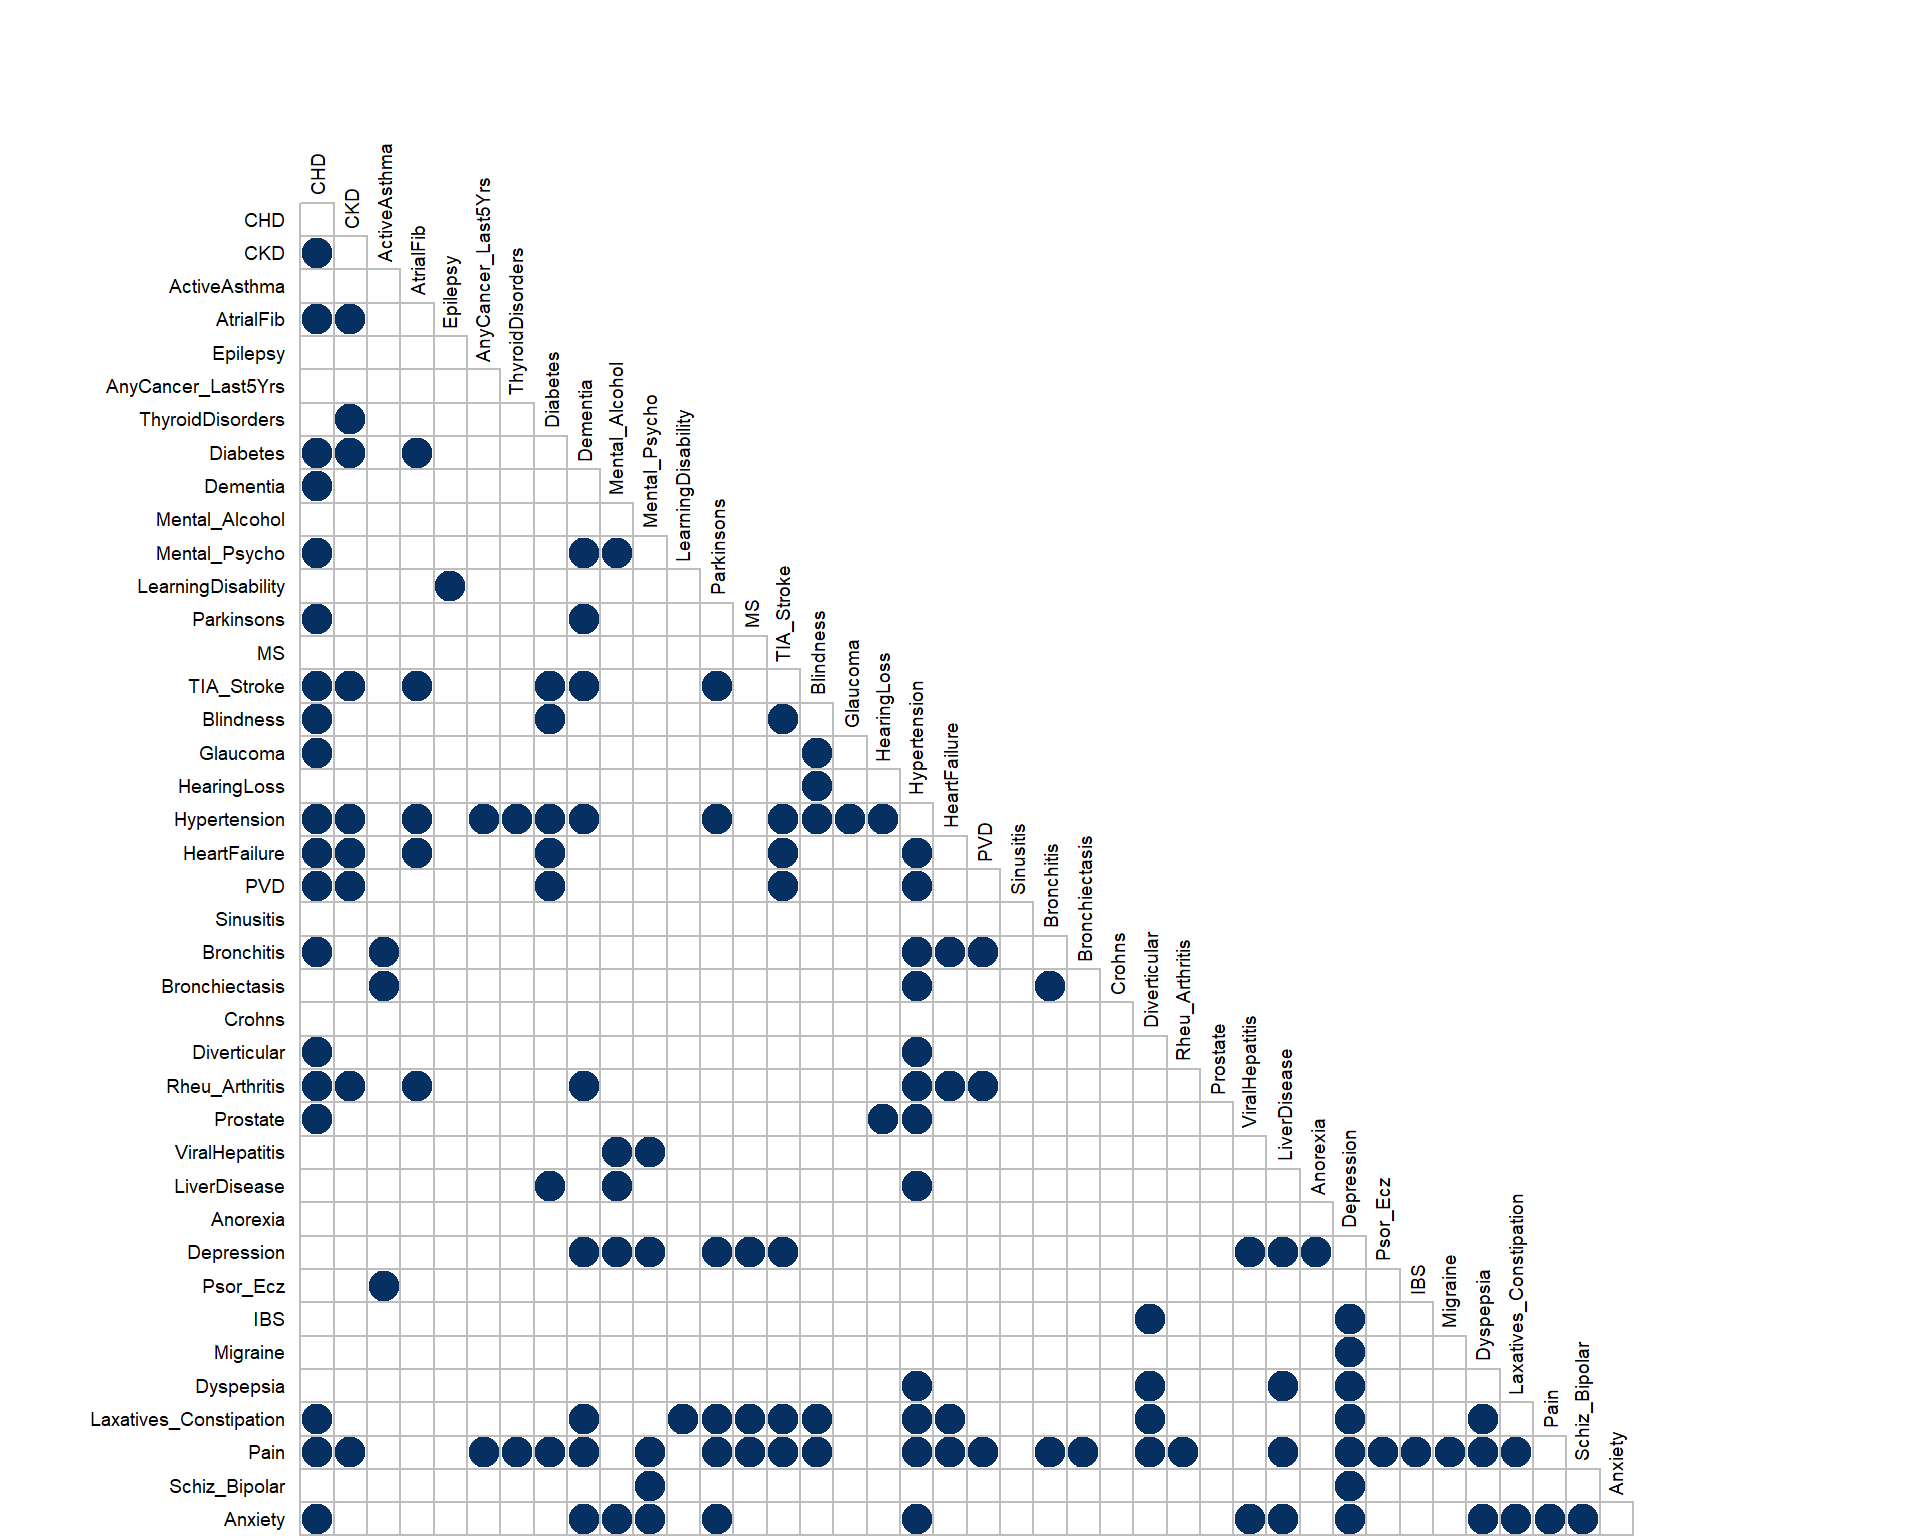
\includegraphics[width=0.9\textwidth]{figures/sd-corrplot.png}
  \caption{Significant Pairwise Correlations}
  \label{fig:corrplot}
\end{figure}

With \(\alpha\) controlled at 0.001, 143 of a possible 780 pairwise
correlations proved to be significant. A matrix showing all
statistically significant correlations is shown in Figure
\ref{fig:corrplot}. The number of expected false positives for 143 pairs
is less than 1.

\subsection{Grouping diseases}\label{subsec:clust-grouping}

Using the ``clumping'' procedure detailed in Ng \citeyearpar{RN72},
Thirty-eight overlapping groups of conditions were found as shown in
Table \ref{tab:overlap}

\begin{table}[]
  \centering
  \caption{Overlapping groups of diseases derived from "clumping" procedure}
  \label{tab:overlap}
  \resizebox{\textwidth}{!}{%
    \begin{tabular}{@{}lll@{}}
    \toprule
    \textbf{Group} & \textbf{Diseases Included} & \textbf{Strength} \\ \midrule
    1 & CHD, CKD, AtrialFib, Hypertension, HeartFailure, Rheu-Arthritis, PVD &        0.2833 \\
    2 & CHD, CKD, AtrialFib, Diabetes, TIA-Stroke, Hypertension, HeartFailure &       0.2806 \\
    3 & CHD, CKD, Hypertension, HeartFailure, Rheu-Arthritis, Pain & 0.2653 \\
    4 & CHD, Hypertension, Prostate & 0.2622 \\
    5 & CHD, CKD, Diabetes, TIA-Stroke, Hypertension, HeartFailure, Pain & 0.259      \\
    6 & CHD, TIA-Stroke, Hypertension, HeartFailure, Laxat-Constip, Pain & 0.2525     \\
    7 & Mental-Alcohol, LiverDisease, Depression, Anxiety & 0.2512 \\
    8 & CHD, Hypertension, HeartFailure, Bronchitis, Pain & 0.2487 \\
    9 & CHD, CKD, Diabetes, TIA-Stroke, Hypertension, PVD, Pain & 0.2348 \\
    10 & CHD, CKD, Hypertension, PVD, Rheu-Arthritis, Pain & 0.2331 \\
    11 & Mental-Alcohol, Mental-Psycho, ViralHepatitis, Depression, Anxiety &         0.2324 \\
    12 & Mental-Psycho, Depression, Schiz-Bipolar, Anxiety & 0.2304 \\
    13 & CHD, Hypertension, Diverticular, Laxat-Constip, Pain & 0.2294 \\
    14 & Depression, Migraine, Pain & 0.2278 \\
    15 & CKD, ThyroidDisorders, Hypertension, Pain & 0.2262 \\
    16 & CHD, Blindness, Glaucoma, Hypertension & 0.2236 \\
    17 & Depression, Dyspepsia, Laxat-Constip, Pain, Anxiety & 0.218 \\
    18 & MS, Depression, Laxat-Constip, Pain & 0.2178 \\
    19 & CHD, Diabetes, TIA-Stroke, Blindness, Hypertension, Pain & 0.2171 \\
    20 & ActiveAsthma, Bronchitis, Bronchiectasis & 0.2166 \\
    21 & CHD, TIS-Stroke, Blindness, Hypertension, Laxat-Constip, Pain & 0.2138 \\
    22 & CHD, Hypertension, PVD, Bronchitis, Pain & 0.2114 \\
    23 & CHD, Dementia, Parkinsons, TIA-Stroke, Hypertension, Laxat-Constip, Pain     & 0.2068 \\
    24 & Dementia, Parkinsons, Depression, Laxat-Constip, Pain, Anxiety & 0.2068      \\
    25 & CHD, Dementia, Hypertension, Rheu-Arthritis, Pain & 0.204 \\
    26 & Diabetes, Hypertension, LiverDisease, Pain & 0.1964 \\
    27 & Dementia, Mental-Psycho, Depression, Pain, Anxiety & 0.1939 \\
    28 & Hypertension, Diverticular, Dyspepsia, Laxat-Constip, Pain & 0.1938 \\
    29 & CHD, Dementia, Parkinsons, Hypertension, Laxat-Constip, Pain, Anxiety &      0.1922 \\
    30 & Hypertension, Bronchitis, Bronchiectasis, Pain & 0.1917 \\
    31 & Blindness, HearingLoss, Hypertension & 0.179 \\
    32 & Dementia, Parkinsons, TIA-Stroke, Depression, Laxat-Constip, Pain & 0.173     \\
    33 & HearingLoss, Hypertension, Prostate & 0.1729 \\
    34 & AnyCancer-Last5Yrs, Hypertension, Pain & 0.1707 \\
    35 & Hypertension, LiverDisease, Dyspepsia, Pain, Anxiety & 0.1593 \\
    36 & Depression, IBS, Pain & 0.1563 \\
    37 & CHD, Dementia, Mental-Psycho, Pain, Anxiety & 0.1385 \\
    38 & Diverticular, IBS, Pain & 0.1226 \\ \bottomrule
    \end{tabular}%
  }
\end{table}

Six diseases; Epilepsy, Learning Disability, Sinusitis, Crohns,
Anorexia, Psoriasis/Eczema did not have strong enough pairwise
correlations to be included in any of the 38 groups. Thirteen
non-overlapping groups were derived from the results of the clumping
method using the algorithm described above and named according to the
characteristics of the member disease in the groups as shown in Table
\ref{tab:no-overlap}.

A further four diseases; Diverticular disease, Prostate, IBS, and
Dyspepsia were excluded from the non-overlapping groups. These four
conditions did not appear in any groups with the diseases with which
they had strongest pairwise correlation, a condition that had to be met
in the first stage of the algorithm described above.

\begin{table}[]
  \centering
  \caption{Non-overlapping groups of diseases derived from Ng algorithm}
  \label{tab:no-overlap}
  \resizebox{\textwidth}{!}{%
  \begin{tabular}{@{}ll@{}}
    \toprule
    \textbf{Disease group name} & \textbf{Diseases included} \\ \midrule
    \textit{Cardiovascular} & CHD, CKD, AtrialFib, Hypertension, HeartFailure,        Rheu-Arthritis, PVD \\
    \textit{Diabetes/Stroke} & Diabetes, Stroke \\
    \textit{Pain/MS} & Laxatives/Constipation, Pain, MS \\
    \textit{Mental Health/Liver} & Mental/Alcohol, Liver Diseases, Depression,        Anxiety \\
    \textit{Psychosis} & Mental-Psycho, Viral Hepatitis \\
    \textit{Sciz/Bipolar} & Sciz-Bipolar \\
    \textit{Migraine} & Migraine \\
    \textit{Thyroid} & Thyroid disorders \\
    \textit{Blindness} & Blindness, Glaucoma \\
    \textit{Respiratory} & ActiveAsthma, Bronchitis, Bronchiectasis \\
    \textit{Neurodegenerative} & Dementia, Parkinson's \\
    \textit{Hearing Loss} & Hearing Loss \\
    \textit{Cancer} & Any Cancer in Last 5 years \\ \bottomrule
    \end{tabular}%
  }
\end{table}

\subsection{Grouping individuals}\label{subsec:clust-clustering}

Individuals were assigned a score depending on the number of diseases
they had in each of the non-overlapping groups according to the criteria
described above. The finite mixture model of multivariate generalised
Bernoulli distributions was then applied to this dataset in order to
identify latent groups of individuals depending on their scores for each
of the 13 groups, based on presence of 30 diseases. BIC scores suggested
the model for nine latent groups had best fit to the data. The
nine-group model was compared with the model with second-lowest value of
BIC, that for eight latent groups. However, despite offering a more
parsimonious solution, the eight-group model did not provide a more
substantive theoretical fit to the data. Thus, the nine-group model was
deemed best fit and analysed further.

Item-response probabilities for the nine-group model are shown in Figure
\ref{fig:item-response}.

\begin{figure}
  \centering
    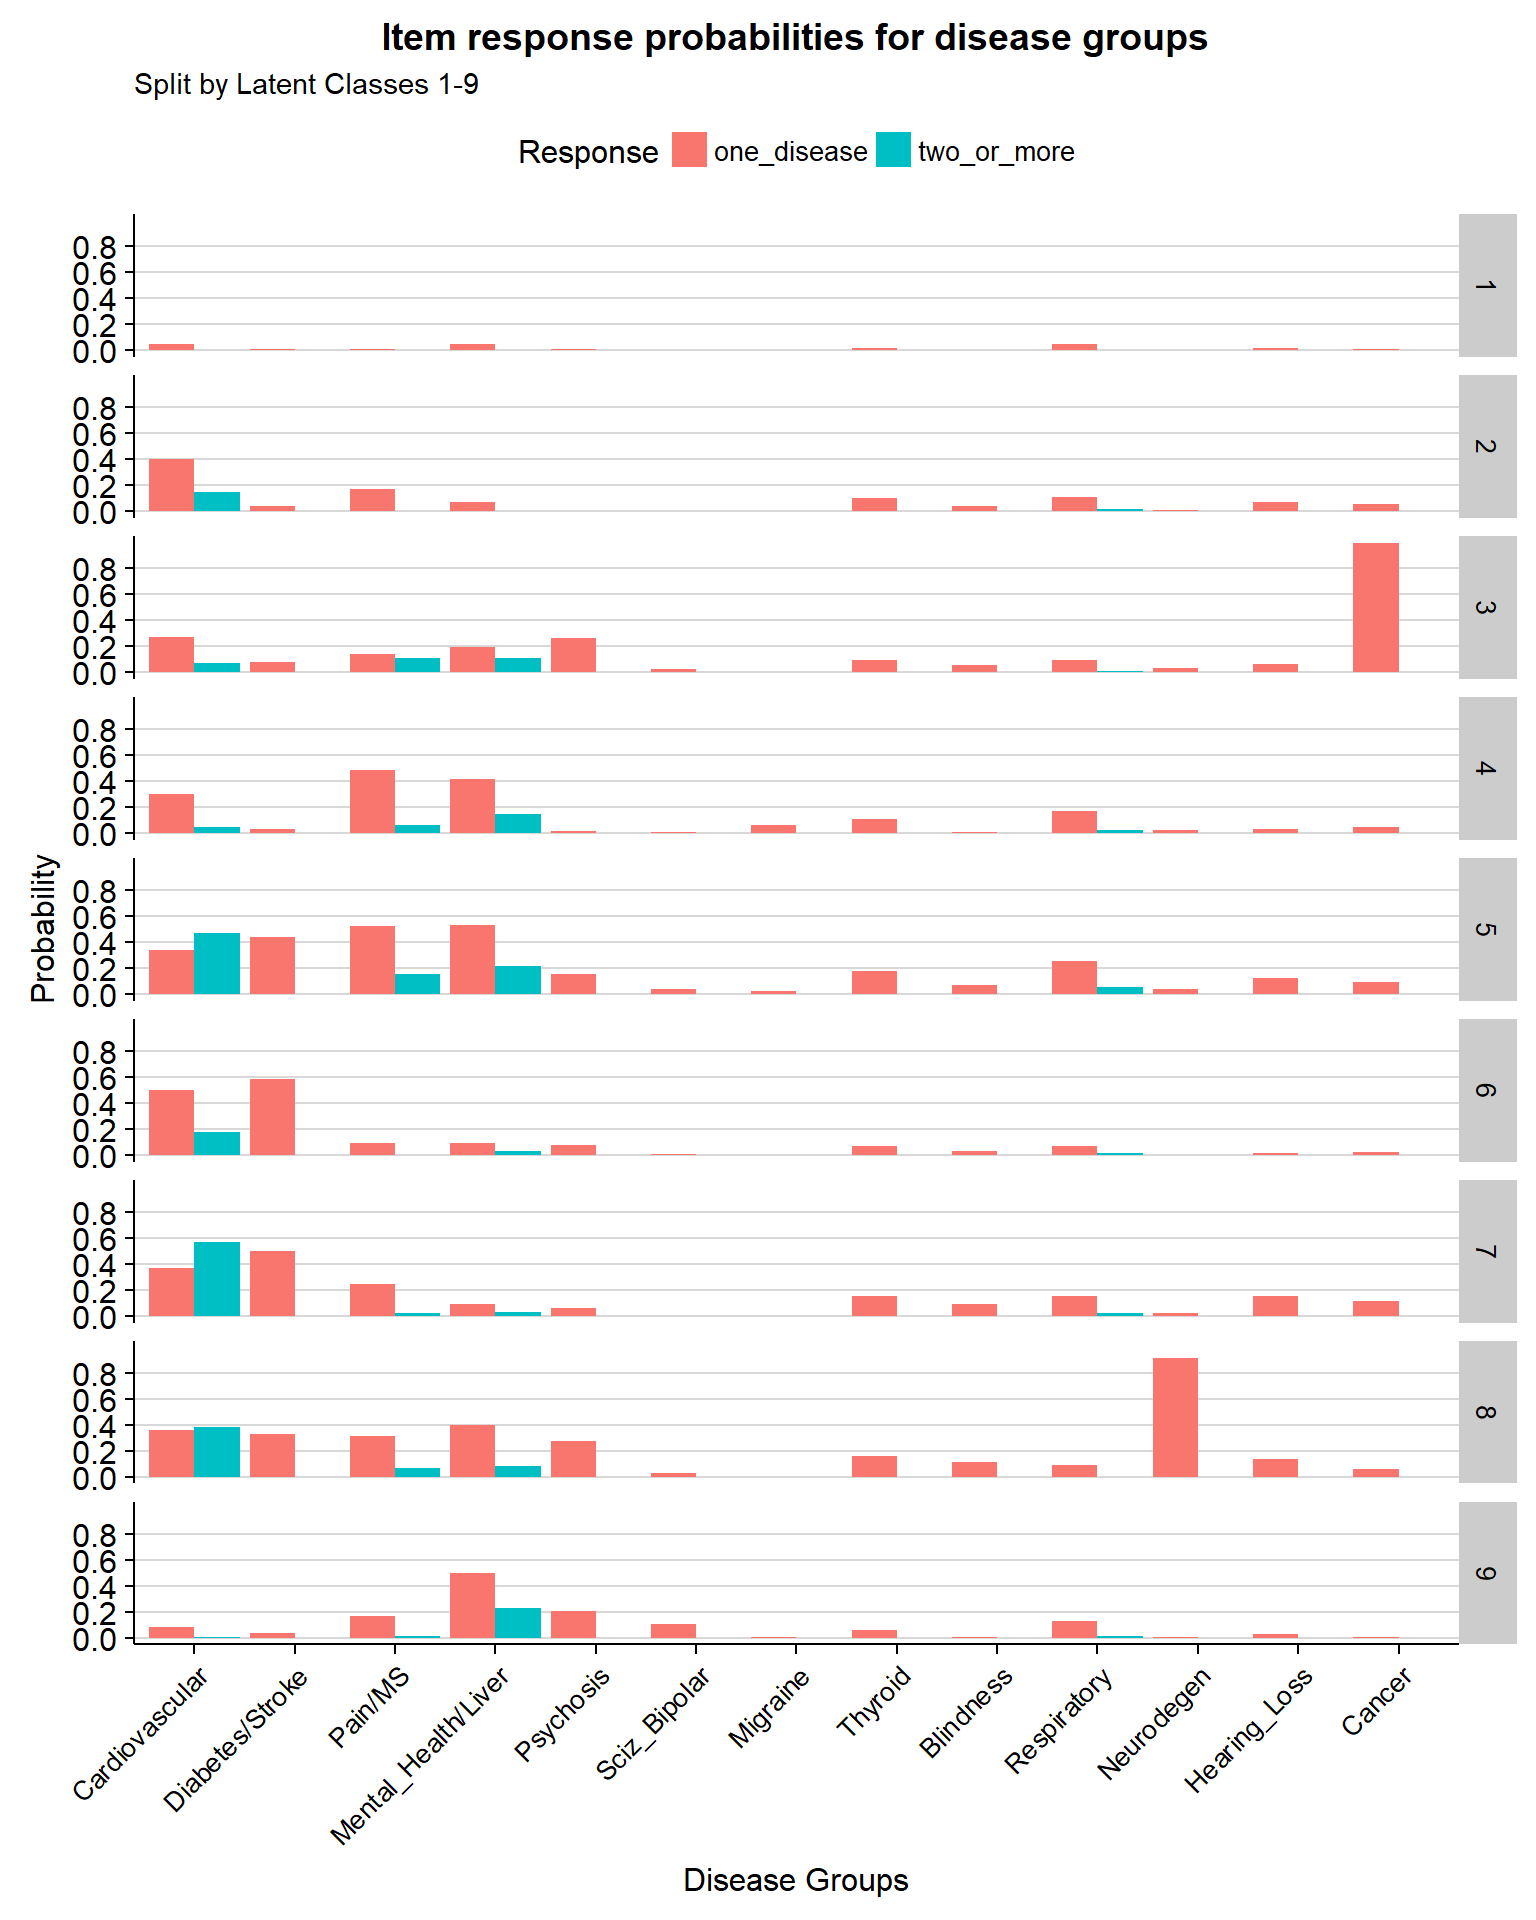
\includegraphics[width=0.9\textwidth]{figures/item-response.png}
  \caption{Item response probabilities for nine latent group model}
  \label{fig:item-response}
\end{figure}

Each latent group was labelled according to these item response
probabilities as follows;

\begin{itemize}
\tightlist
\item
  Latent Group 1. \textbf{Well}. High probabilities of having no
  diseases in any of the groups.
\item
  Latent Group 2. \textbf{Cardiovascular only}. Item response in this
  Latent group have more than 50\% chance of having at least 1 condition
  from the Cardiovascular group. High probabilities of having no
  diseases in any of the other groups.
\item
  Latent Group 3. \textbf{Cancer}. Individuals in this group have almost
  100\% probability of having had cancer in last 5 years. Weak
  probabilities across some other groups.
\item
  Latent Group 4. \textbf{Mental Health/Pain} High probability of having
  at least one diseases from Pain/MS group and at least one disease from
  Mental Health/Liver group.
\item
  Latent Group 5. \textbf{Mental and Physical Multimorbidity} High
  probabilities of having at least 1 cardiovascular, diabetes/stroke,
  Pain/MS, and Mental health/Liver disease. This group also has the
  highest probability across latent groups for having 1 respiratory
  disease.
\item
  Latent Group 6 \textbf{Physical Multimorbidity} High probability of a
  least one cardiovascular disease and one of Diabetes/Stroke.
\item
  Latent Group 7. \textbf{Physical multimorbidity (Strong Cardio)}.
  Similar to Latent group 6 but individuals in this group are more
  likely to have 2 or more cardiovascular diseases.
\item
  Latent Group 8. \textbf{Dementia with Mental/Physical MM} Individuals
  in this latent group have almost 100\% probability of having dementia
  or Parkinson's. Also highly likely to have at least one Cardiovascular
  disease and mildly raised probability of having mental health or
  psychosis diseases.
\item
  Latent Group 9. \textbf{Mental Health only}. High probability of
  having a least 1 of the Mental Health/Liver group diseases. Also
  mildly raised probabilities in the Psychosis and Sciz\_Bipolar groups.
\end{itemize}

Proportionate size of each of the assigned latent variable groups is
shown in Figure \ref{fig:group-props}.

\begin{figure}
  \centering
    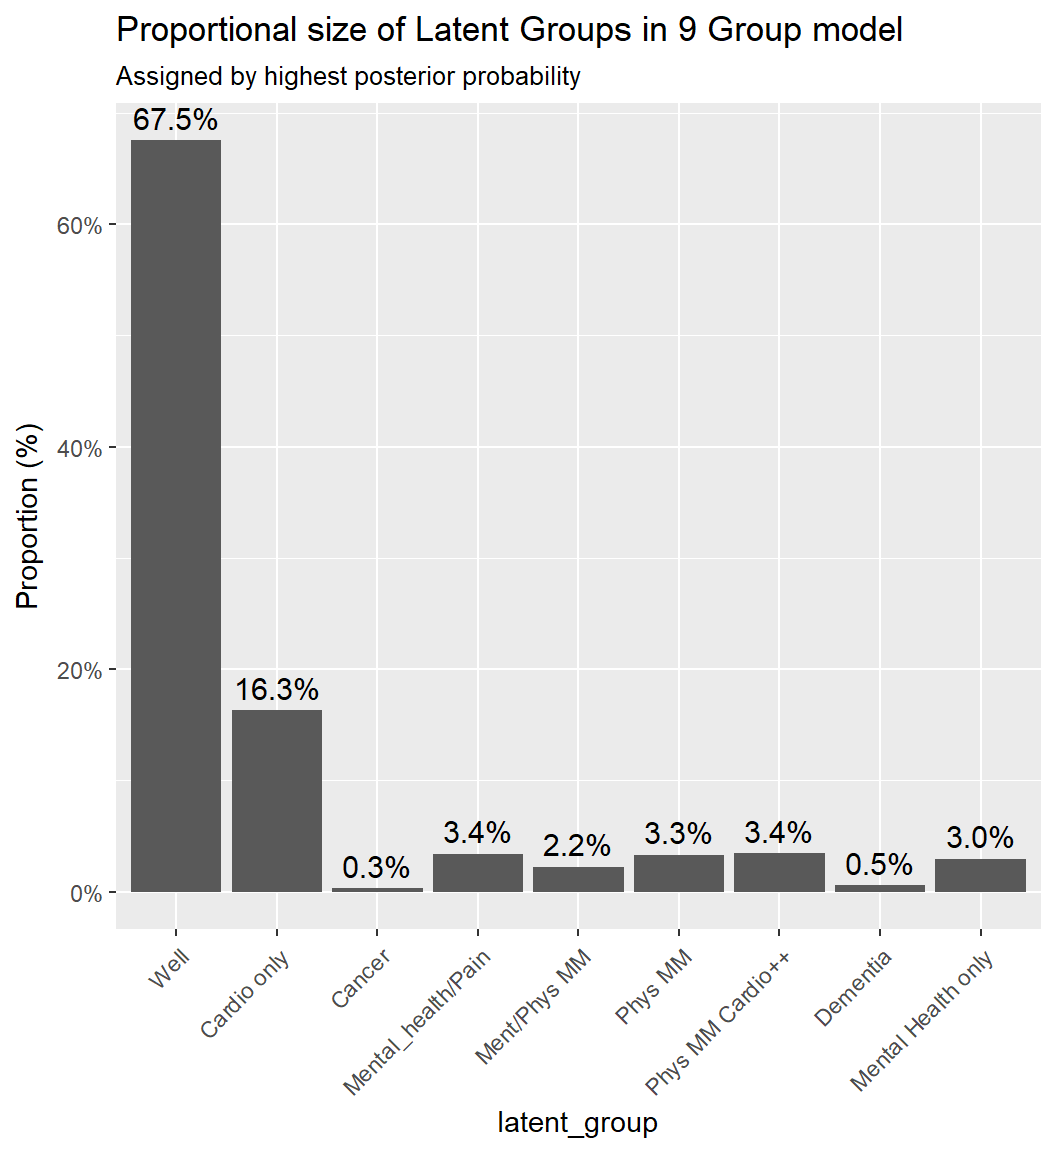
\includegraphics[width=0.9\textwidth]{figures/props.png}
  \caption{Latent Group Proportions}
  \label{fig:group-props}
\end{figure}

The ``Well'' latent group was by far the largest group with almost 70\%
of individuals within it. The other groups formed much smaller
proportions of the data.

\subsection{Sociodemographic breakdown of latent groups}\label{subsec:clust-ses}

Each of the Histograms of Age for each of the latent groups shown in
Figure \ref{fig:lg-by-age} show variation in distribution. The ``Well''
and ``Mental Health only'' groups have a much younger age distribution
compared to the other groups. The ``Dementia'' group has a much older
distribution.

\begin{figure}
  \centering
    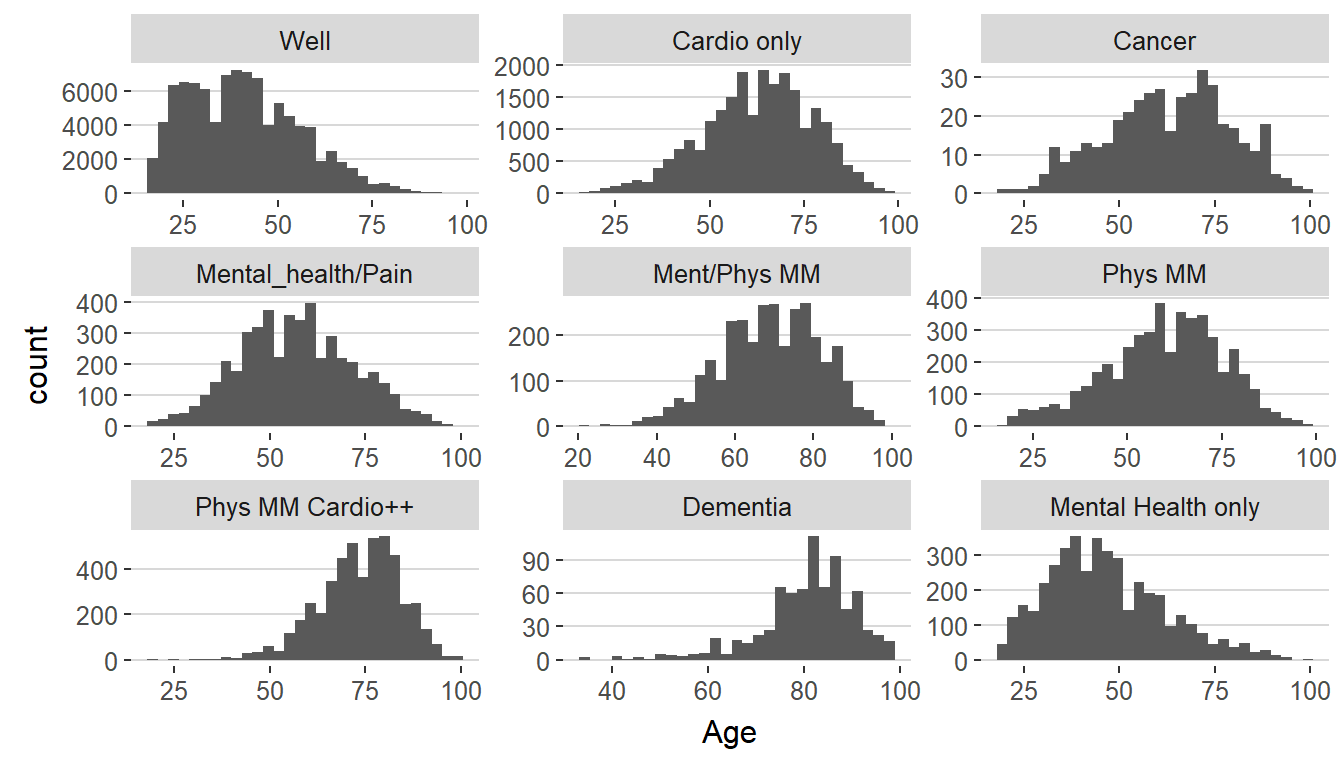
\includegraphics[width=0.9\textwidth]{figures/lg-by-age.png}
  \caption{Histograms of Age, by Latent Group}
  \label{fig:lg-by-age}
\end{figure}

Figure \ref{fig:lg-by-sex} shows higher proportions of males in the
``Physical MM'' latent group. The ``Well'' and ``Physical MM high
Cardio'' groups have even splits by gender. All other groups have higher
proportions of females.

\begin{figure}
  \centering
    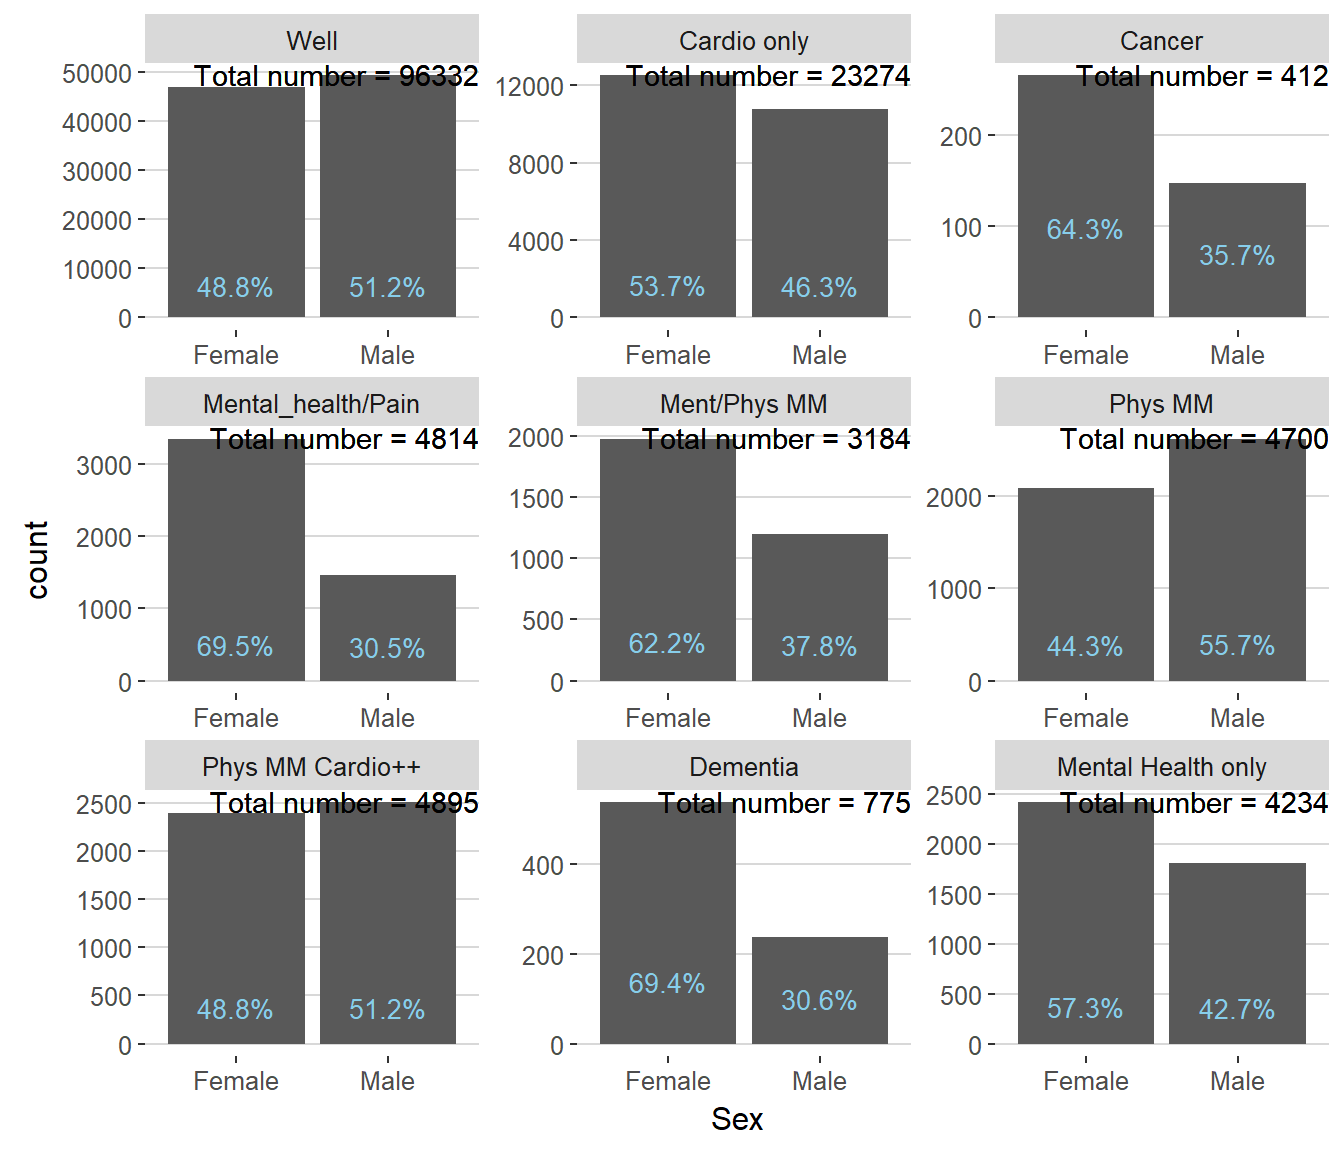
\includegraphics[width=0.9\textwidth]{figures/lg-by-sex.png}
  \caption{Count of Sec, by Latent Group - with Proportions}
  \label{fig:lg-by-sex}
\end{figure}

Figure \ref{fig:lg-by-dep} shows distribution of deprivation across
latent groups by Carstairs Decile. There are clear gradients in the
``Mental Health \& Pain'', ``Ment/Phys MM'', and ``Mental Health only''
groups with much higher numbers of people in Decile 10 (most deprived)
areas.

\begin{figure}
  \centering
    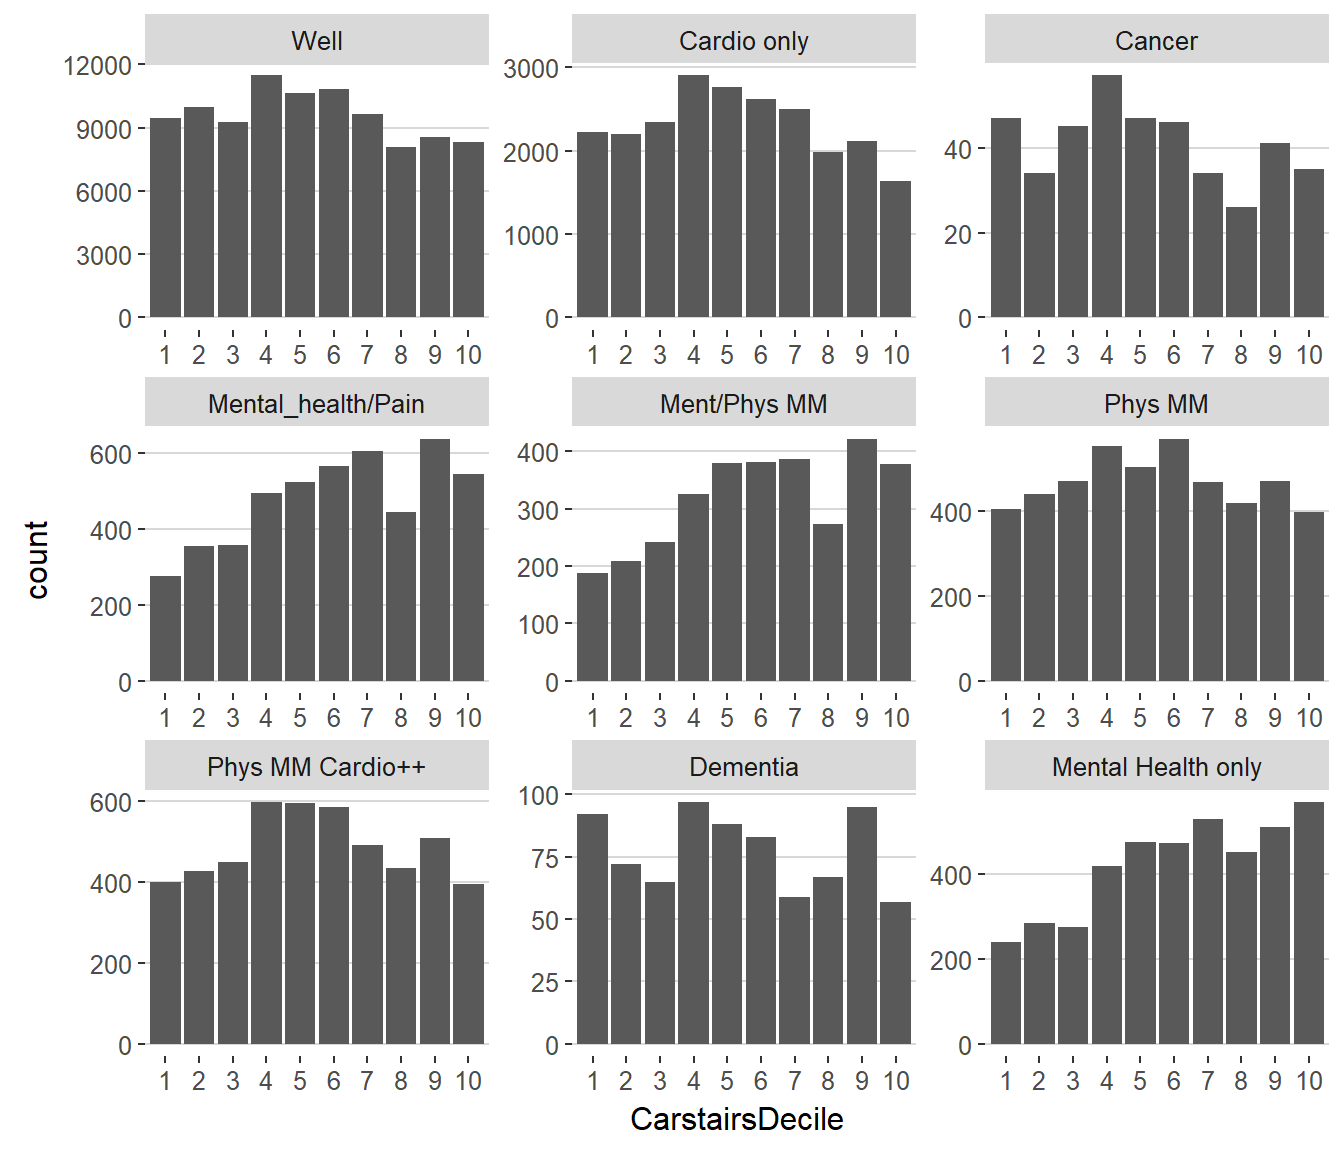
\includegraphics[width=0.9\textwidth]{figures/lg-by-dep.png}
  \caption{Count of Carstairs Decile, by Latent Group}
  \label{fig:lg-by-dep}
\end{figure}

\FloatBarrier

\section{Discussion}\label{sec:clust-discussion}

When proposing the two-way clustering method, Ng \citeyearpar{RN72}
applied the technique to Australian survey data of 24 self-reported
diseases from n=8841 respondents. These were ``clumped'' into nine
non-overlapping groups of diseases with four latent groups of
individuals being identified by the mixture model. Given the different
classification of diseases, the nature of how data were collected, and
the different populations, it is unsurprising that results from the
present study are markedly different. What is of interest is whether the
technique provided a meaningful representation of the data which can be
used to improve the understanding of multimorbidity within this
population.

The first step of the two-way clustering technique resulted in 13
non-overlapping groups being formed. As a result of this process, ten of
the diseases recorded in the dataset were excluded from the final
groups. Six diseases; Epilepsy, Learning Disability, Sinusitis, Crohns,
Anorexia, and Psoriasis/Eczema did not have strong enough pairwise
Somer's D correlation statistics with any other disease to be included
in the non-overlapping ``clumping'' procedure. A further four diseases;
Diverticular, Prostate, IBS, and Dyspepsia did not appear in any
non-overlapping group with the disease with which they had the strongest
Somer's D correlation. Identifying which diseases do not co-occur at
non-random levels is a particularly interesting finding and adds to the
debate about which diseases should be included in any multimorbidity
measure.{[}be explicit -- do you think this suggests we shouldn't count
these 10 in any MM measure and, if so, why? -NB{]} Of the 40 diseases
present in the SPICE-PC dataset, in this analysis, only 30 diseases
co-occurred with enough statistical power to be added to non-overlapping
disease groups and considered in the mixture model.

Past research has highlighted associations between; mental health and
thyroid problems, mental health and pain, and diseases associated with
the metabolic syndrome \citep{RN98}. As shown in figure 1, there is no
pairwise correlation between any mental health diseases and thyroid
disorders in the present study. Pain is associated with a large number
of conditions, including mental health diseases. Diseases associated
with metabolic syndrome such as, hypertension, coronary heart disease,
diabetes, stroke, and heart failure all show correlations with each
other to varying degrees. Prados-Torres et al \citeyearpar{RN98} also
identified associations between Chronic Obstructive Pulmonary Disease
(COPD) and Gastroesophageal reflux disease (GORD) with mental health
diseases. No associations with between any respiratory disease and
mental health diseases is apparent in figure 1. The SPICE-PC dataset
does not record GORD, however Dyspepsia may be considered a similar
diagnosis and has pairwise correlations with both Depression and
Anxiety.

The non-overlapping disease groups were named according to the
characteristics of the diseases present in each, however many diseases
appeared in groups that may not come from similar aetiology. The groups
reflect diseases that commonly co-occur and therefore do not always fit
into clinically recognisable groups. Individuals are scored as to the
number of diseases they have from each group. This results in a loss of
some information but the advantage of this method is that it reduces the
number of variables in the dataset making the likelihood of identifying
a good mixture model much more likely.

Applying a mixture model of multivariate generalised Bernoulli
distributions to these 13 non-overlapping disease groups identified nine
latent groups as described above. These groups are clinically
recognisable with some showing presence of diseases from only one
disease group and others illustrating a more multimorbid population.
Clear distinctions between mental and physical disease are made enabling
individuals to have diseases from both groups. In their systematic
review of clustering studies of multimorbidity, Prados-Torres et al
\citeyearpar{RN98} found that included studies reported between three
and twenty diseases clusters. From these they found three most common
groups of diseases; cardiovascular, mental health, and musculoskeletal.
Latent groups in the current study also contain cardiovascular and
mental health elements, although they do not reflect any groups that
could be identified as musculoskeletal.

Clear sociodemographic patterns were identified in the latent groups.
Those classified as belonging to a latent group with mental health
involvement such as; mental health/pain, mental and physical
multimorbidity, or mental health only, were more likely to be female and
from lower deprivation deciles. Two similar latent groups; physical
multimorbidity and physical multimorbidity high cardiovascular, had
clear age differences with the former more likely to have younger male
individuals assigned to it. These findings are similar to simple
analyses of the same dataset which identified those in the most deprived
areas being more likely to develop physical and mental health
multimorbidity 10-15 years earlier than their more affluent peers
\citep{RN33}.

\subsection{Limitations}\label{subsec:clust-limitations}

The two-step method proposed by Ng \citeyearpar{RN72} enables reduction
of dimensions in datasets with large numbers of disease variables making
model good identification of mixture models more likely. This, however,
results in a loss of detail making interpretation of results more
difficult. Report of the item-response probabilities shown in figure 4
identifies that individuals have a probability of having none, one, or
two of the diseases in any group. It is impossible to identify exactly
which diseases. Hypertension with 13.4\% of individuals is the highest
reported disease in the SPICE-PC . To what degree this accounts for
individuals having one disease in the cardiovascular group across latent
classes is unknown.

This is particularly a problem as the non-overlapping groups formed by
the two-way clustering method do not always follow recognised clinical
groupings. For example, Rheumatoid arthritis is found in the
cardiovascular group despite being a connective tissue disorder. It is
the only disease in the group that does not directly affect the
cardiovascular system. The reason it is found in this group may be due
to the association of increased NSAID use with cardiovascular outcomes
(ref) resulting in frequent co-occurrence. As some latent groups are
classified as ``Cardiovascular only'', there is a possibility that small
numbers of people with only Rheumatoid Arthritis are misclassified.
{[}This is could be down to nomenclature and I maybe need to revisit
group names. It does not get rid of the problem that for the group with
high probs for the cardio/rheum disease we can't distinguish which
disease the individual has{]}

When clustering individuals, fitting a finite mixture model of
multivariate generalised Bernoulli distributions makes the assumption
that the indicator variables used to identify latent groups are
independent. In a dataset containing medical conditions such as
e.g.~Hypertension and Coronary Heart Disease, or Atrial Fibrillation and
Stroke, this assumption is clearly violated. However, ignoring the
independence assumption for multivariate categorical variables often
results in better fit than when more complicated techniques are applied
to account for non-independence of indicator variables
\citep{RN72, RN298, RN297}.

Results presented here account for 10\% of the SPICE-PC dataset due to
the heavy computational requirements of fitting the finite mixture
model. Confirmation of results on the whole dataset is required.

\subsection{Future research}\label{subsec:clust-future}

Sociodemographic comparison in the current study was limited to
visualisation of histograms. More detailed reports of measures of
central tendency and comparison of latent groups with sociodemographic
variables such as Carstairs decile with logistic regression is
warranted. SPICE-PC data also contains variables on lifestyle factors
such as smoking status and alcohol intake. These variables should be
included in further comparisons.

A further calculation offered in the two-way clustering technique
\citep{RN72} is the calculation of a multimorbidity score to each latent
group and to each individual in the dataset based on their disease
profile and posterior probabilities. Such as score would be continuous
in nature and would offer the benefit of comparison with
sociodemographic variables such Carstairs score or Age. Such comparisons
would be amenable to well-recognised regression techniques.

Part 1 of the two-step method involves reducing the dimensions of the
dataset to be amenable to mixture modelling. Using the outcome of this
first step, the non-overlapping groups, Ng's technique for clustering
individuals should be compared to Latent Class Analysis which is also a
suitable technique for the nature of the data \citep{RN291}. In
supplementary material, NG \citeyearpar{RN72} compared his two-step
method with Latent Profile Analysis and found it inferior to the
two-step method. Latent Profile Analysis is a mixture model for
continuous indicator variables \citep{RN291} and would not be suitable
for the SPICE-PC dataset.

\section{Conclusion}\label{sec:clust-conclusion}

A novel two-step method for clustering health conditions and individuals
was applied to large, population representative, dataset of
administrative primary care data. The method found 10 of the 40
conditions in the dataset did not co-occur with other diseases strongly
enough to included in further analysis. Thirty conditions were
``clumped'' into 13 groups of commonly co-occurring conditions and
individuals in the dataset were assigned a score depending on the number
of disease within each group they had. From this information nine latent
groups of individuals were identified with a finite mixture model. These
groups reflected varying degrees of physical, mental and physical/mental
multimorbidity and showed sociodemographic patterning.

\FloatBarrier
\newpage
\fancyhead[CO,CE]{Chapter 4. Measuring Multimorbidity}

\chapter{Data}\label{ch:data}

\section{Infrastructure}\label{sec:infrastructure}

\begin{itemize}[noitemsep]
\item Describe record linkage
\item Overview of Scottish linkage
\end{itemize}

\subsection{Urban Big Data Centre}\label{subsec:ubdc}

Describe UBDC (one of three - ADRN and Farr also)

\subsection{NHS National Services Scotland}\label{subsec:edris}

Describe eDRIS

\subsection{National Records of Scotland}\label{subsec:nrs}

Describe NRS

\section{Data Sources}\label{sec:sources}

\subsection{Social Care}\label{subsec:source-sc}

Descibe Social Care Survey

\subsection{Population Spine and Death records}

via eDRIS or direct NRS?? - demography and geography also.

\subsection{Prescribing Information System}

Describe PIS

\subsection{Unscheduled Care Data}

Describe USC data mart

\section{Information Governance}\label{sec:ig}

\subsection{Research Approvals Commitee}\label{subsec:rac}

UBDC RAC process

\subsection{Public Benefit and Privacy Panel}\label{subsec:pbpp}

PBPP Process

\subsection{Ethics}\label{subsec:ethics}

College ethics and waivers

\subsection{Data sharing agreement}\label{subsec:dsa}

DSA description

\section{Safe Haven environment}\label{sec:safe-haven}

describe safe haven

\section{Timeline}\label{sec:timeline}

Describe timeline of approvals process - major hurdles and barriers.

\FloatBarrier
\newpage
\fancyhead[CO,CE]{Chpater 5. Renfrewshire Council Pilot Project}

\chapter{Methods}\label{ch:methods}

\section{Cohort}\label{sec:cohort}

Describe the cohort - why it was chosen. How it was constructed

\section{Linkage process}\label{sec:linkage}

Detail of linkage process with diagramme. In-depth detail here.

\section{Summary measures}\label{sec:summaries}

\subsection{Social Care Survey}\label{subsec:scs-summs}

Which variables were used and how summarised and cleaned (i.e.~telecare
as categorical etc.)

with reference to chapter \ref{ch:renfrew} and measure of hours of
social care

\subsection{Prescribing Information Service}\label{subsec:pis-summs}

How PIS data was summarised and measures chosen

\subsection{Demographic, geographic, and deaths information}\label{subsec:nrs-summs}

Which Local Authority? Which SIMD data?

\subsection{Unscheduled care measures}\label{subsec:usc-summs}

How was usc data wrangled? Which summary measures were chosen?

\section{Statistical methods}

Which summary and model statisitics were used to answer research
questions.

\FloatBarrier
\newpage
\fancyhead[CO,CE]{Chapter 6. Linked Data Quality Assessment}

\chapter{Renfrewshire Council Pilot Project}\label{ch:renfrew}

\section{Background}\label{sec:renf-background}

Pilot project to get first look at social care data to determine
structure and definitions. Main linkage project to use cross-sectional
social care data -
\emph{is this reflective of social care provision throughout the year?}
Also able to attach datazone and demogrpahic variables - is there
variation in amounts of care across these variables? (potentially drop
this second part)

\subsection{Aims}\label{subsec:renfrew-aims}

\begin{itemize}
\tightlist
\item
  Describe the temporal variation in levels of care within financial
  years
\item
  Describe variation in social care provision in Renfrewshire Council
  area by Age, Gender, and socioeconomic position. (potentially drop)
\item
  Assess the quality of social care data for research purposes
  (potentially drop)
\end{itemize}

\subsection{Research Questions}\label{subsec:renfrew-qs}

\begin{enumerate}[noitemsep]
\item How does social care use vary within and across financial years 2006/07 - 2015/16?
\item Is there variation in the amount of social care delivered in the Renfrewshire Council area by Age, Gender, and Socioeconomic position? (?drop)
\end{enumerate}

\section{Methods}\label{sec:renf-methods}

Describe manipulation of variables to produce summary stats.

Describe which methods used to summarise variation in care

Link to RAC approval process described in chapter \ref{ch:data} section
\ref{subsec:rac}. Also link to use of safe haven described in section
\ref{sec:safe-haven}. Re-mention ethics. Note that PBPP not required fir
this pilot

\section{Results}\label{sec:renf-results}

Tables and graphs of results with description

\begin{itemize}[noitemsep]
\item Number of individuals
\item Dropped records
\item Per year breakdown of individuals
\item Age - Gender - SIMD breakdown
\item Mean hrs of homecare - median, range, interquartile range
\item Average difference in hrs homecare (census week) and three previous quarters
\item Average difference in hrs homecare (census week) and three following quarters
\end{itemize}

\section{Discussion}\label{sec:renf-discuss}

Implications - particular focus on variation in care throughout the year
and whether care provided in a census week is a robust measure for
research purposes (based on Renfrew results)

Limitations - One council only. Different collection and reporting
methods across LAs etc etc.

\section{Conclusion}\label{sec:renf-conc}

\FloatBarrier
\newpage
\fancyhead[CO,CE]{Chapter 6. Access to Social Care}

\chapter{Results}\label{ch:results}

\section{Introduction}\label{sec:social-care-intro}

Link to chapter \ref{ch:intro} and chapter \ref{ch:lit-review} re aims
and research questions. Chapter \ref{ch:methods} for methods

\section{Data Linkage}\label{sec:res-linkage}

Percent matches etc.

\section{Characteristics of cohort}

Long table

\begin{itemize}[noitemsep]
\item n
\item Age - mean, median, range IQR.
\item Sex
\item Local Authority
\item SIMD
\end{itemize}

\section{Social care and multimorbidity}\label{sec:sc-mm}

\begin{itemize}[noitemsep]
\item Any SC by number of meds
\item Hrs homecare by number of meds
\item Telecare by number of meds
\item etc.
\end{itemize}

\section{Geographic variation in social care}

Accounting for MM

\section{Social care, multimorbidity, and unscheduled health care use}

\begin{itemize}[noitemsep]
\item National picture
\item broken down by LA
\item broken down by HB
\end{itemize}

\section{Social Care, multimorbidity, and mortality}

\begin{itemize}[noitemsep]
\item National picture
\item broken down by LA
\item broken down by HB
\end{itemize}

\section{Discussion}\label{sec:social-care-discuss}

\section{Conclusion}\label{sec:social-care-conclu}

\FloatBarrier

\FloatBarrier
\newpage
\fancyhead[CO,CE]{Chapter 7. Social Care and Health Outcomes}

\chapter{Conclusion}\label{ch:conclusion}

Reccomendations :-

\begin{itemize}
\item Standardised score reflecting need/frailty/vulnerability required to accurately assess access to care (OECD pp181)
\item disaggregate SCS a little - distinguishing reablement and intermediate care from LTC important!
\item Measure outcomes relevent to social care (falls etc OECD 2013 pp59) OR link to outcome data e.g. preventable admission data, hip fracture data??
\item Consider other forms of admin data to help with this e.g. Attendance Allowance?? - Problem being coverage
\end{itemize}

\FloatBarrier
\newpage
\fancyhead[CO,CE]{Appendices}

\appendix
\chapter{Title A}

Testing, testing. One-two, one-two.

\chapter{Title B}

Let's see what this looks like

\FloatBarrier
\clearpage

\addcontentsline{toc}{chapter}{Bibliography}

\bibliography{thesis}


\end{document}
